\documentclass[iop]{../emulateapj}

% these lines seem necessary for pdflatex to get the paper size right
\pdfpagewidth 8.5in
\pdfpageheight 11.0in

% for the red MarginPars
\usepackage{color}

% some extra math symbols
\usepackage{mathtools}

% allows Greek symbols to be bold
\usepackage{bm}

% allows us to force the location of a figure
\usepackage{float}

% allows comment sections
\usepackage{verbatim}

% allows in-document links; see http://www.astrobetter.com/blog/2014/09/29/latex-hyperref-and-emulateapj/
\usepackage[backref,breaklinks,colorlinks,citecolor=blue]{hyperref} 
\usepackage[all]{hypcap} %Links go to figures;breaks on deluxetables       
\renewcommand*{\backref}[1]{[#1]}

% Override choices in \autoref
\def\sectionautorefname{Section}
\def\subsectionautorefname{Section}
\def\subsubsectionautorefname{Section}

% MarginPars
\setlength{\marginparwidth}{0.75in}
\newcommand{\MarginPar}[1]{\marginpar{\vskip-\baselineskip\raggedright\tiny\sffamily\hrule\smallskip{\color{red}#1}\par\smallskip\hrule}}

\newcommand{\evm}{{(-)}}
\newcommand{\evz}{{(\circ)}}
\newcommand{\evp}{{(+)}}
\newcommand{\enu}{{(\nu)}}

\newcommand{\msolar}{\mathrm{M}_\odot}

% Software names
\newcommand{\boxlib}{\texttt{BoxLib}}
\newcommand{\castro}{\texttt{CASTRO}}
\newcommand{\wdmerger}{\texttt{wdmerger}}
\newcommand{\python}{\texttt{Python}}
\newcommand{\matplotlib}{\texttt{matplotlib}}
\newcommand{\yt}{\texttt{yt}}

\begin{document}

%==========================================================================
% Title
%==========================================================================
\title{Double White Dwarf Mergers on Adaptive Meshes\\ I. Methodology and Code Verification}

\shorttitle{WD Mergers I. Methodology}
\shortauthors{Katz et al. (2015)}

\author{Max P. Katz, Michael Zingale, Alan C. Calder, F. Douglas Swesty, Ann S. Almgren, Weiqun Zhang}
%==========================================================================
% Abstract
%==========================================================================
\begin{abstract}
The Type Ia supernova progenitor problem is one of the most perplexing and 
exciting problems in astrophysics, requiring detailed numerical modelling to 
complement the observations of these explosions. One possibility that has 
merited recent theoretical attention is the white dwarf merger scenario.
This can naturally explain many of the observed characteristics of 
Type Ia supernovae, as well as their distribution in time and space.
However, to date there have been few fully self-consistent simulations 
of binary white dwarf systems using mesh-based hydrodynamics, 
relative to other methods. This is the first paper in a series designed to 
describe simulations of these systems using a hydrodynamics code with 
using the adaptive-mesh refinement approach. In this paper we describe our numerical 
methodology and discuss our implementation in the code \castro. \castro\ 
solves the Euler equations of hydrodynamics 
and the Poisson equation for self-gravity. Standard techniques for 
coupling gravitation and rotation forces to the hydrodynamics do 
not do an adequate job conserving the total energy of the system, 
but recent advances in the literature have made advances on this 
problem and we discuss our implementation here. We also run an 
extensive set of test problems to verify that our software can sufficiently
model a system where large amounts of mass are advected on the computational 
domain over very long timescales. Future papers in this series will describe
our treatment of the initial conditions of these systems, and will 
examine the early phases of the merger to determine its viability
for triggering a thermonuclear detonation.

\end{abstract}
\keywords{hydrodynamics - methods: numerical - supernovae: general - white dwarfs}

%==========================================================================
% Introduction
%==========================================================================
\section{Introduction}

Type Ia supernovae (SNe Ia) are currently some of the most exciting
events to study in astrophysics. These bright, brief pulses of light
in the distant universe have led to a number of important discoveries
in recent years, including the discovery of the accelerated expansion
of the universe \citep{perlmutter1999,riess1998}. However, their
origin is shrouded in mystery. It has long been expected that these
events arise from the thermonuclear explosions of white dwarfs
\citep{hoyle_fowler:1960}, but the cause of these explosions is
uncertain. In particular, it is not clear what process causes the
temperatures in these white dwarfs to become hot enough for explosive
burning of its constituent nuclei. The model favored initially by the
community was the so-called single-degenerate (SD) model
\citep{whelan_iben:1973}. Accretion of material from a companion star
such as a red giant would cause the star to approach the Chandrasekhar
mass, and in doing so the temperature and density in the center would
become sufficient for thermonuclear fusion to proceed. However, in
recent years many alternative progenitor models have been discussed. A
leading candidate for explaining some or most of these explosions is
the double-degenerate (DD) model, in which two white dwarfs merge and
the merged object reaches the conditions necessary for a thermonuclear
ignition \citep{ibentutukov:1984,webbink:1984}. Another is the double
detonation scenario, where accretion of material onto a
sub-Chandrasekhar white dwarf would lead to a detonation inside the
accreted envelope, and this would send a compressional wave into the
core of the star that would trigger a secondary detonation. A recent
review of the progenitor models can be found in
\citet{hillebrandt:2013}.

There are several observational reasons why double-degenerate systems
are a promising progenitor system for at least a substantial fraction
of normal SNe Ia. No conclusive evidence exists for a surviving
companion star of a SN Ia; this is naturally explained by the DD model
because both WDs are likely to be destroyed in the merger
process. Similarly, pre-explosion images of the SN Ia systems have
never clearly turned up a companion star, and in some cases a large
fraction of the parameter space for the nature of the companion star
is excluded. Additionally, not enough progenitor systems are seen for
the SD case to match the observed local SN Ia rate, whereas the number
of white dwarf binaries may be sufficient to account for this
rate. Finally, the DD model can naturally explain the fact that many
SNe Ia are observed to occur at very long delay times after the stars
were formed, since the progenitor systems only become active once both
stars have evolved off the main sequence. A thorough review of the
observational evidence about SNe Ia and further discussion of these
ideas can be found in \cite{maoz:2014}.

The first attempts to model the results of the merger process came in the
1980s. \cite{nomotoiben:1985} demonstrated that off-center carbon
ignition would occur in the more massive white dwarf as it accreted
mass near the Eddington rate from the less massive white dwarf
overflowing its Roche lobe. \cite{saionomoto:1985} tracked the
evolution of the flame and found that it propagated quiescently into
the center, converting the carbon-oxygen white dwarf into an
oxygen-neon-magnesium white dwarf. This would then be followed by
collapse into a neutron star -- a result with significantly different
observational properties compared to a SN Ia. This scenario, termed
accretion-induced collapse, would be avoided only if the accretion
rate were well below the Eddington rate. \cite{tutukov_yungelson:1979}
observed that this could happen if the mass loss from the secondary
was higher than the Eddington rate and thus the accreted material
formed an accretion disc, which might rain down on the primary more
slowly. The main finding was that double degenerate systems would not
obviously lead to Type Ia supernovae.

Three-dimensional simulations of merging double degenerate systems were 
first performed by \citet{benz:1990}, who used the smoothed particle
hydrodynamics (SPH) method to simulate the merger process. This was 
followed later by a number of authors 
\citep{rasio_shapiro:1995,segretain:1997,guerrero:2004,yoon:2007,loren-aguilar:2009,raskin:2012}.
The main finding of these early 3D SPH simulations was that if the 
lower-mass star (generally called the ``secondary'') was
close enough to the more massive star (the ``primary'') to begin mass
transfer on a dynamical time scale, the secondary completely disrupted
and formed a hot envelope around the primary, with a
centrifugally-supported accretion disk surrounding the core and
envelope. Carbon fusion might commence in the disk, but not at a 
high enough rate to generate a nuclear detonation. \cite{mochkovitch_livio:1990} 
and \cite{livio:2000}  also observed that turbulent viscosity in this disk 
would be sufficiently large for angular momentum to be removed from the 
disk at a rate high enough to generate the troublesome accretion 
timescales discussed by \cite{tutukov_yungelson:1979}. Based on this
evidence, the review of \cite{hillebrandtniemeyer2000} argued that the
model was only viable if the accretion-induced collapse problem could
be avoided. Later work by \cite{shen:2012} and \cite{schwab:2012} used
a more detailed treatment of the viscous transport in the outer
regions of the remnant and found that viscous dissipation in the centrifugally
supported envelope would substantially heat up the envelope on a  
viscous timescale, but their simulations still led to off-center carbon
burning. \cite{vankerkwijk:2010} argued that equal-mass mergers would
lead to the conditions necessary for carbon detonation in the center
of the merged object, but \cite{shen:2012} questioned this for similar
reasons related to how viscous transport would convert rotational
motion into pressure support. \cite{zhu:2013} followed this with an
expanded parameter space study and argued that many of their
carbon-oxygen systems had the potential to detonate. The study of the
long-term evolution of the remnants is thus still an open subject of
research.

A recent shift in perspective on this problem started around 2010.
\cite{pakmor:2010} used the SPH method to study the merger of 
equal-mass ($0.9\ \msolar$) carbon-oxygen white dwarfs and found 
that a hotspot was generated near the surface of the primary 
white dwarf. They argued that this region had a temperature 
and density sufficient to trigger a thermonuclear
detonation. They inserted a detonation which propagated throughout 
the system. They found that the result would observationally 
appear as a subluminous Type Ia supernova. This was the first time 
a DD simulation successfully reproduced at least some characteristics of a SN
Ia. \cite{pakmor:2011} tried a few different mass combinations and
found empirically that this would hold as long as the secondary was at
least 80\% as massive as the primary. These events, where the merger
process resulted in the detonation of the system during the merger
coalescence -- avoiding the much longer time-scale evolution -- were
termed ``violent'' mergers.

Around the same time, however, \cite{guillochon:2010} and
\cite{dan:2011} pointed out that the previously mentioned simulations 
generally shared a significant drawback, which was that their initial conditions
were not carefully constructed. \cite{motl:2002}, \cite{dsouza:2006},
and \cite{motl:2007} (the first three-dimensional grid-based
simulations of mass transfer in binary white dwarf systems) pioneered
the study of looking at the long-term dynamical evolution of binary
white dwarf systems after constructing exact equilibrium initial
conditions. Earlier work placed the stars too close together 
and ignored the effects of tidal forces that change the shape of the 
secondary, leading to the merger
happening artificially too quickly. When the initial conditions are
constructed in exact equilibrium, the system can be stable for tens of
orbital periods, substantially changing the character of the mass
transfer phase. However, one limitation of this series of studies is
that the authors used a polytropic equation of state and thus could
not consider nuclear reactions. \cite{guillochon:2010} and
\cite{dan:2011} improved on this using a realistic equation of state,
a nuclear reaction network, and a similar approach to the equilibrium
initial conditions, and found substantial agreement with the idea that
mass transfer occurs in a stable manner over tens of orbital
periods. They also found that, assuming the material accreted onto the
surface of the primary was primarily helium, explosive surface
detonations would occur as a result of accretion stream instabilities
during the mass transfer phase prior to the full merger. This could
trigger a double-detonation explosion and thus perhaps a SN Ia.

The latest developments have resulted in some possible areas of convergence.
\cite{pakmor:2012} performed a merger scenario
with a $1.1\ \msolar$ and $0.9\ \msolar$ setup, with better treatment
of the initial conditions, and indeed found that the merger process
happened over more than ten orbits. Nevertheless, they still determined
that a carbon-oxygen detonation would occur, in line with their
earlier results. \cite{moll:2014} was also able to find a detonation
in a similarly massive system. Very recently, \cite{kashyap:2015} 
found that a detonation occurred in a similarly massive system. Notably,
the detonation occurred self-consistently and did not need to be inserted 
by hand. \cite{dan:2012} and \cite{dan:2014} performed a large sweep 
of the parameter space for merger pairs and
found that pure carbon-oxygen systems would generally not lead to
detonations and violent mergers except for the most massive
systems. They did find that for systems containing helium, many
would detonate and potentially lead to SNe Ia, either through the
aforementioned instabilities in the accretion stream, or during the
contact phase, similar to the violent carbon-oxygen
mergers. \cite{pakmor:2013} added a thin helium shell on their primary
white dwarf, and found that this robustly led to a detonation of the
white dwarf. For now there is preliminary support for the hypothesis
that systems with helium shells (or helium WDs), and very massive carbon-oxygen binaries,
could robustly lead to events resembling SNe Ia.

Given the above, why is another approach using a different simulation
code warranted? First and foremost, reproducibility of the results
across simulation codes and algorithms is important for gauging
confidence in this result. Most of the existing results that study 
the viability of double degenerate systems as progenitors for
Type Ia supernovae (that is, including a realistic 
equation of state and nuclear reactions) have
used the SPH method. SPH codes have a number of features which do aid
them in the study of these systems, such as excellent conservation of
angular momentum. However, the question of whether a prompt detonation
in a merger actually happens depends in detail on the nature of the
gas at the interface between the two stars, which is at much lower
density than the rest of the stellar material. The SPH codes use
uniform mass particles, so their effective resolution is
\textit{lowest} at the stellar surface. In contrast, a grid-based code
with adaptive mesh refinement can zoom in on the regions where
hotspots will develop, while also maintaining high enough resolution
in the high-density regions to adequately capture the large-scale mass
transfer dynamics. However, there are also outstanding questions of
convergence in SPH (e.g.\ \citealt{zhu_SPH:2014}) and whether the method
correctly captures fluid instabilities. This is an important question
for white dwarf mergers because of the likely importance small-scale
instabilities will have on the evolution of the low-density gas at the
primary's surface. The pioneering work of \cite{agertz:2007} compared
grid and SPH codes and found some important differences. Most relevant
for this discussion is that the SPH codes could not adequately handle
mixing from the Kelvin-Helmholtz instability in the test they
propose. As pointed out by \cite{price:2008}, this is not a result of
SPH being inherently unable to model this instability, but instead it
is attributed to the fact that the standard SPH evolution equations do
not have a mechanism for capturing discontinuities in internal
energy. \citeauthor{price:2008} showed that the addition of an
artificial thermal conductivity can dramatically improve the ability
of the SPH codes to exhibit this instability. There have since been a
number of other papers discussing this issue, but to our knowledge
none of these improvements have yet been incorporated into an SPH
model of a WD merger. Another reason for caution is that other than the
most recent results of \cite{kashyap:2015}, no simulation has self-consistently
resulted in a thermonuclear detonation. Reproducibility of the detonation 
through direct numerical simulation is critical for building 
confidence in this progenitor model.

This is the first in a series of papers designed to address these
outstanding theoretical issues for white dwarf mergers. This work will
discuss the verification of our hydrodynamics code for simulating
these events. Later efforts will look at the initial conditions of the
system, the robustness with which a hotspot is found from which a
detonation could occur, and the importance of the initial white dwarf
models, which should be more sophisticated than simple carbon-oxygen
mixtures and in principle should use results from modern stellar
evolution calculations. \autoref{sec:Numerical Methodology}
%\hyperref[sec:Numerical Methodology]{Section \ref*{sec:Numerical Methodology}}
describes our code and why it can provide useful results compared to
other methodologies used for this problem. 
\autoref{sec:initial_models} describes the method we use for setting up a
binary white dwarf simulation. \autoref{sec:Tests} discusses a few
test problems that we use to demonstrate that our code accurately
solves the equations of fluid dynamics. \autoref{sec:Performance}
demonstrates that the software scales well for supercomputer
applications. Finally, \autoref{sec:Conclusions and Discussion}
recaps what we have shown and highlights some of the future work we
plan to do.

%==========================================================================
% Numerical Methodology
%==========================================================================
\section{Numerical Methodology}\label{sec:Numerical Methodology}

To study the white dwarf merger problem, we use the grid-based
hydrodynamics code \castro\footnote{\castro\ can be obtained at \url{https://github.com/BoxLib-Codes/Castro}.} \citep{castro}.
\castro\ solves the Euler
equations, along with the inclusion of optional modules for gravity,
nuclear reactions and thermodynamics. \castro\ is based on the \boxlib
\footnote{\boxlib\ can be obtained at \url{https://github.com/BoxLib-Codes/BoxLib}.}
adaptive-mesh refinement (AMR) framework \citep{rendleman:2000}, which
represents fluid data on a mesh where regions of interest have higher
spatial resolution. \castro\ is highly parallel and is designed for
large-scale use on modern supercomputers; see 
\autoref{sec:Performance} for information on how \castro\ performs for our
problem. The next few subsections describe our approach to each of the
physics components used in this work. We direct the reader to the
original code paper for a full description of \castro's approach to
solving the equations of hydrodynamics. In this work, we report mainly
on the changes we have made to the code since its original release,
for the purpose of approaching this problem.

\subsection{Hydrodynamics}\label{sec:Hydrodynamics}

The Euler equations for hydrodynamics (in the absence of source terms) in conservative form are:
\begin{align}
  \frac{\partial \rho}{\partial t} &= -\bm{\nabla} \cdot (\rho \mathbf{u}) \label{eq:euler_density}\\
  \frac{\partial \rho \mathbf{u}}{\partial t} &= -\bm{\nabla} \cdot (\rho \mathbf{u}\mathbf{u}) - \bm{\nabla}p \label{eq:euler_momentum}\\
  \frac{\partial \rho E}{\partial t} &= -\bm{\nabla}\cdot(\rho\mathbf{u}E + p\mathbf{u}). \label{eq:euler_energy}
\end{align}
Here $\rho$ is the mass density, $\mathbf{u}$ is the fluid velocity
vector, $p$ is the pressure, and $E = \mathbf{u}^2 / 2 + e$ is the
total specific energy, where $e$ is the internal (thermal) specific
energy (energy per unit mass).

We use the unsplit piecewise-parabolic method (PPM) solver in \castro\
to advance the hydrodynamics system in time \citep{ppmunsplit}.  A
number of changes were made to the solver, which are detailed in the
Appendix.  These changes bring the algorithm more in line with that of
\cite{ppm}. \castro\ as originally released featured a slightly modified
version of the higher resolution limiters of
\cite{colella_sekora:2008}, which can be accessed in the code using
\texttt{castro.ppm\_type = 2}. The advantage of this limiter is that
it preserves physical extrema rather than clipping them off as in the
original approach of \cite{ppm}. However, we found these limiters to
be unsatisfactory for our problem. There are many regions in our
problem with large density gradients (such as the interface between
the star's atmosphere and the ambient gas outside of it) and in these
regions the algorithm can yield negative densities. This often results
from the limiters interpreting these gradients as being true
minima. As a result, we use the original limiter, which is strictly
monotonicity preserving in the parabolic profiles it generates; this
is activated with \texttt{castro.ppm\_type = 1}.

A related issue that required a code improvement is that in cases of
large density gradients such as the edge of a star, it is possible to
generate negative densities in zones even with the more strongly
limited PPM. This can occur if a region of large density is moving
away from an ambient zone at relatively large speeds; then the net
density flux in the ambient zones can be large enough to unphysically
drag the density below zero. In practice, this will occur at the
trailing edge of a star that is moving across a grid. In such a
situation, there are two main approaches one could take: either
explicitly introduce a positivity-guaranteeing diffusive flux, or
reset the characteristics of the affected zone. We choose the latter
approach. Even though it is non-conservative, it preserves a
characteristic we value, which is to keep the edge of the stars
relatively sharp, as they physically should be. Since the mass of the
affected zones is typically already fairly low, this should not
seriously affect the energy conservation properties of our
simulation. Our strategy for a reset is as follows: when the density of 
a zone is below a pre-determined density floor (which is typically 
$10^{-5}\ \text{g cm}^{-3}$ for our stellar simulations), we look
at all adjacent zones and find the zone with the highest density.
If it is above the density floor, then we set the field values 
(density, momentum, energy, and temperature) of the
resetted zone to be exactly equal to the field values of this 
adjacent zone. If no adjacent zone reaches the density floor, then
the zone is set to the density floor, and given a temperature equal 
to the temperature floor for our simulations (which is typically 
$10^{5}\ \text{K}$ for our stellar simulations). We then recompute 
the thermodynamics to be consistent with these values. The 
velocity of the zone is set to zero. This latter approach will only
occur in very rare situations, and is mainly there as a safeguard.

\castro's approach to adaptive mesh refinement, based on its underlying
\boxlib\ framework, is to refine zones based on certain user-specified
criteria that tag regions of interest for higher spatial
resolution. Data is represented on one of a number of AMR levels,
where each level corresponds to a set of zones at the same resolution,
which covers a subset of the domain covered by the level immediately
below it. We typically call the level 0 grid the \textit{coarse} grid,
which has the lowest spatial resolution. Each finer, higher-level grid
has a higher resolution than the grid below it by some integer factor
$N$, which is restricted to be $N = 2\ \text{or}\ 4$ in the code. The
zones are strictly contained within the rectangular extent of the
underlying coarser zones (the code is not restricted to representing
only Cartesian geometries, but we use a Cartesian mesh with uniform
spacing in each dimension for the present study). For the time
evolution of the AMR system we use subcycling, where each AMR level is
advanced at a different timestep and a correction step is applied at
the end to synchronize the various levels. Generally the number of
subcycled timesteps is equal to the jump in refinement between levels,
so for example on a grid with three levels and two jumps of four in
refinement, the level 2 zones will have 16 times higher spatial
resolution than the coarse grid and there will be 16 level 2 timesteps
per level 0 timestep.

The boundary conditions on the hyperbolic system are simply
zero-gradient zones that allow material to flow directly out of the
domain. Using AMR, we make the coarse grid large enough that the
boundaries are relatively far from the region of interest. This
ensures that any boundary effects do not pollute the inner region
where the stars will eventually make contact.  We further make the
restriction that refined grids cannot reach the domain boundary.

\subsection{Microphysics}

The equation of state (EOS) for our simulations is the Helmholtz EOS
\citep{timmes_swesty:2000}. This models an electron-positron gas of
arbitrary relativity and degeneracy over a wide range of temperatures
and densities. Thermodynamic quantities are calculated as derivatives
of the Helmholtz free energy, and the values are interpolated from a
table. The natural variables of the Helmholtz free energy are
temperature and density, and calling the EOS is simplest in this
form. However, in hydrodynamics we often have the density, and
internal energy as independent variables, and we want to obtain the
temperature, pressure, and other quantities. To do this, we employ a
Newton-Raphson iteration over the temperature (given some sufficient
starting guess) until we find the temperature that corresponds to the
desired internal energy. Sometimes this process fails to converge and
the iterative value approaches zero. In these cases we employ a
``floor'' that limits how low the temperature can go (typically 
$10^5$ K). There is a choice here how to proceed: we can either
assign this floor value to the temperature and let that zone be
thermodynamically inconsistent (the original behavior in \castro), or
we can adjust the internal energy to be thermodynamically consistent
with the temperature, at the cost of violating energy conservation. We
have found in some test problems of strong one-dimensional shocks that reach 
the temperature floor that the latter yields more accurate results. 
However, allowing the equation of state call to update the 
internal energy can actually result in significant changes to the 
total energy of the system over long periods of time, 
due not just to resets in low-density zones but also to small 
inconsistencies between the energy given to the EOS and the energy 
that is consistent with the returned temperature. These inconsistencies
are dependent on the threshold we set that determines how close the 
returned energy should be to the original input energy. While this 
threshold is typically very small in an individual zone (a relative 
difference of $10^{-8}$ by default in \castro), over time and given 
a large number of zones, this can result in a significant energy 
drift. This is a serious enough problem that we opt for the energy 
conserving approach for our simulations.

\castro\ has the ability to do both nuclear reactions and radiative 
transport (in the flux-limited diffusion approximation). For all simulations 
in this paper we do not enable either, and will delay discussion of 
these modules until a later paper in this series.

\subsection{Gravity}
\label{sec:gravity}

We solve the Poisson equation for self-gravity for our problem,
\begin{equation}
  \nabla^2 \Phi(\mathbf{x}) = 4\pi G\, \rho(\mathbf{x}),
\end{equation}
where $\Phi$ is the gravitational potential, $G$ is the gravitational
constant, and $\rho$ is the mass density.\footnote{In the \castro\ code, the 
right-hand side is negated and therefore $\Phi$ is positive. We use the 
sign convention that is typical for astrophysics in this paper. 
When $\Phi$ appears in the code it is negated to compensate for this.} 
The solution of this equation in \castro\ is described in \cite{castro}, and
consists of both level and composite solves, and a final
synchronization at the end.

\subsubsection{Coupling to Hydrodynamics}\label{sec:gravity_hydro_coupling}

The effect of gravity on the hydrodynamical evolution is typically
incorporated by the use of a source term for the momentum and energy
equations. In a finite volume methodology, the momentum source term 
as traditionally written appears in integral form as
\begin{equation}
  \left.\frac{\partial (\rho \mathbf{u})}{\partial t}\right|_{\text{grav}} = \frac{1}{\Delta V} \int \rho \mathbf{g}\, dV
\end{equation}
and for the energy source term the analogue it is
\begin{equation}
  \left.\frac{\partial (\rho E)}{\partial t}\right|_{\text{grav}} = \frac{1}{\Delta V} \int \rho \mathbf{u}\cdot\mathbf{g}\, dV \label{eq:cell_center_gravity_source}.
\end{equation}
Here $\Delta V$ is the cell's volume.
In most hydrodynamics codes these are discretized as $\rho\,
\mathbf{g}$ and $\rho\, \mathbf{u}\,\cdot\mathbf{g}$, respectively, 
where $\rho$, $\mathbf{u}$, and $\mathbf{g}$ 
are evaluated at the zone center. 

There are two ways that these source terms enter the hydrodynamics update.
First, during the hydrodynamics update, we alter the edge states that enter
into the determination of the fluxes. (This only applies for the momentum source term;
the gravitational force does not directly do work on the internal energy, which is used 
to infer the pressure.) To second order in space and time, 
this can be done using the cell-centered
source term evaluated at time-level $n$. The details of this are described in 
the appendix. Second, after the hydrodynamics step, we add the time-centered source terms
to the state. First we will describe how we do this for the momentum,
and then we will describe our approach for the energy. This discussion will be somewhat detailed.
However, we believe that the attention is necessary because of the importance of accuracy
in the gravitational source terms for our problem. The stability of the white dwarf binary
system is dependent in large part upon accurate coupling of the hydrodynamics and gravity;
an error in this approach could lead to, for example, a spurious mass transfer episode
that might lead us to very different conclusions about the long term stability of such a system.
Such considerations are generally unimportant for spherically-symmetric single star calculations,
but are of the utmost importance in a simulation where the global gravitational field can change 
quite significantly over the course of the simulation.

In a system with self-gravity, total momentum is conserved if the spatial domain
includes all of the mass of the system. This must be the 
case because each mass element exerts an equal and opposite gravitational force 
on every other mass element. However, the standard approach does not necessarily
guarantee that momentum is conserved numerically. We cannot represent a vacuum state 
in our code, so there is a small but non-zero density on the edge of the grid. 
This allows momentum to leak out of the domain even if the gravitational source term 
is written in an explicitly conservative manner. To see this, one can write the 
density in terms of the potential and then consider its spatial discretization. For simplicity,
we will consider one spatial dimension.
\begin{align}
  -\rho_{i}  \frac{d\Phi_{i}}{dx} &= -\frac{1}{4\pi G} \frac{d^2\Phi_i}{dx^2} \frac{d \Phi}{dx} \notag \\
  &= -\frac{1}{4\pi G} \left[\frac{\Phi_{i-1} - 2 \Phi_{i} + \Phi_{i+1}}{\Delta x^2}\right] \left[ \frac{\Phi_{i+1} - \Phi_{i-1}}{2\Delta x} \right] \notag \\
  &= -\frac{1}{8\pi G \Delta x^3} \left[ \Phi_{i+1}^2 - \Phi_{i-1}^2 - 2\Phi_i\left(\Phi_{i+1} - \Phi_{i-1}\right) \right] \label{eq:momentum_discretization}
\end{align}
It is easy to verify that adding the source terms two cells to the left
and right of this zone will result in complete cancellation of the source terms.
However, if the potential if non-zero outside of the domain, then there will be
momentum lost or gained from the grid, which will be encapsulated in the ghost cells
just outside the domain. In addition, when we replace the Laplacian above by the full
three-dimensional stencil including the $y$ and $z$ derivatives, and depending on the
discretization these will not be cancelled at all. This latter problem can be resolved by
writing the momentum update in an explicitly conservative way.

\citet[Chapter 4]{shu:1992} observes that it is possible to describe the source term 
for the momentum equation by taking the divergence of a gravitational stress tensor,
\begin{equation}
  G_{ij} = -\frac{1}{4\pi G}\left(g_i g_j - \frac{1}{2}|\mathbf{g}|^2\delta_{ij}\right).
\end{equation}
The momentum equations are then written explicitly in conservative form.
The flux at any zone boundary is added to one cell and
subtracted from another, so that the total momentum in the domain interior stays constant to
within numerical roundoff error. This result can be derived by analytically recasting 
\autoref{eq:momentum_discretization}. In the continuum limit, the two momentum
formulations are identical. Thus the latter has been advocated by, for example, 
\cite{jiang:2013} for the ATHENA code. However, in a finite discretization 
the divergence of the gravitational acceleration is no longer guaranteed to equal
the zone density. In particular, we find that the mixing of the gravitational components
means that the truncation error in the gravitational field can lead to large errors
that imply a density much different than the zone's actual density. This is especially
problematic in a simulation with a low-density ambient medium, where even a small error 
in the momentum update can lead to large changes in a zone's momentum. By continuing to explicitly
use the cell density in the momentum update, we can avoid this possibility: the size of the update
will always be suitably small if the zone's density is small. Thus for our simulations
we continue to use the standard source term for the momentum.

Time centering of this source term is done in \castro\ using a predictor-corrector approach.
At the start of a coarse grid timestep, we solve the gravitational potential for the density $\rho^n$.
We then add to the momenta a prediction of the source term that is first-order accurate in time, 
$\Delta t\, \rho^n\, \mathbf{g}^n$. After the hydrodynamics update, we recalculate
the gravitational potential based on the new density, $\rho^n$, and then add 
$-(\Delta t/2) \rho^n \mathbf{g}^n + (\Delta t/2) \rho^{n+1} \mathbf{g}^{n+1}$ to the momenta.

For the energy equation, the central challenge is to write down a form of the 
discretized energy equation that explicitly conserves total energy when 
coupled to gravity. When gravity is included, the total energy is
\begin{equation}
  \rho E_{\text{tot}} = \rho E + \frac{1}{2}\rho\Phi = \frac{1}{2}\rho \mathbf{u}^2 + \rho e + \frac{1}{2}\rho\Phi, \label{eq:total_energy_gravity}
\end{equation}
where $\rho E$ is the total gas energy from the pure hydrodynamics equation,
and the factor of $1/2$ in the gravitational energy term is necessary
for simulations with self-gravity to prevent double-counting of
interactions.

Historically many simulation codes with gravity have not used a conservative formulation 
of the energy equation, but it is straightforward to do so. In particular, conservation of 
total energy requires only that a change in gravitational energy is compensated for by a 
change in gas energy, and that energy changes due to mass transfer are explicitly and 
exactly tracked. At each zone face in a given timestep, there is some transfer of mass $\Delta \rho$ between 
the zones adjacent to that face, which is governed by the continuity equation. Suppose the 
transfer of mass is positive to the right, and the face is located at the (one-dimensional)
index $i-1/2$. Energy is transferred because an amount of mass $\Delta \rho_{i-1/2}$ moves from 
potential $\Phi_{i-1}$ to potential $\Phi_{i}$; if these potentials are different, it requires some 
work exerted by or on the zone to push the mass to this different potential energy. Therefore 
the net change of gravitational energy is $\left[(1/2)\Delta \rho_{i-1/2} (\Phi_{i} - \Phi_{i-1})\right]$,
and if total energy is conserved, then the zone must have a change in gas energy 
$(\rho E)$ that is equal in magnitude and opposite in sign to the change in potential energy. 
Thus the update in a zone for the total energy that conserves $(\rho E_{\text{tot}})$ is:
\begin{equation}
  \Delta (\rho E) = -\frac{1}{2}\sum_{f} \Delta \rho_{f} (\Phi_{f+1/2} - \Phi_{f-1/2}),\label{eq:grav_energy_conservation_update}
\end{equation}
where the sum is over the cell faces $f$ and the indices $f+1/2$ and $f-1/2$ refer to 
the zone centers immediately to the left and right in the direction perpendicular to the face.
Note that while total energy is conserved, the gas energy is not: this does not have the 
telescoping property of a flux formalism where energy gained by one zone is lost by another. 
The energy is being exchanged with a potential field that responds indirectly when the mass moves.

Now the change in the mass $\Delta \rho_{f}$ is proportional to the mass flux through the surface with area $\Delta A$:
\begin{equation}
  \Delta \rho_f = \frac{\Delta t}{\Delta V} (\Delta A\, \rho v_{f}),\label{eq:mass_transfer}
\end{equation}
So as long as we record these fluxes through the zone faces after coming out of the hydrodynamics step, 
we are able to conserve the total energy completely (except for any energy loss or gain through 
physical domain boundaries). In order for the method to be second-order accurate in time, 
no change is needed to the fluxes since those are already time-centered 
in the hydrodynamics update, so we need only to use a time-centered $\Phi$ (which can be computed 
by averaging the time-level $n$ and $n+1$ potentials; we already have the latter because \castro\ 
re-computes the potential at the new time after the hydrodynamics step, and we can apply this energy 
at the end of the timestep).

As observed by \cite{arepo}, when examining \autoref{eq:mass_transfer} one can see the relationship 
between this method and the more common (non-conservative) approach of evaluating the change in 
gas energy using the work done $(\mathbf{v} \cdot \rho \mathbf{g})$ by the gravitational force at the 
cell center. Analytically this form expresses the same core idea via the work-energy theorem, and its 
major flaw is that it evaluates the energy change at the cell center when in fact the mass transfer is 
happening at the cell edges, and the energy change is actually partially compensated by the potential 
in the adjacent zone that the mass is moving to. This is important enough that for simulations where the 
potential can change substantially over the course of the evolution, massive amounts of energy can be lost. 
This standard approach is therefore unacceptable in the case of a problem like white dwarf mergers, and 
the fix to this energy leaking -- evaluating the energy transfer at the six zone faces instead of 
the single zone center -- has a very minor cost in terms of code complexity and computational time.

It is worth pointing out that while \autoref{eq:grav_energy_conservation_update} was correctly obtained 
by \cite{arepo} (and indeed that is the inspiration for this approach), there is a subtle error in that derivation. 
Their argument was that if we integrate the work done over the volume of the zone, this volume integral can be 
converted into a surface integral by use of the divergence theorem (see their Equation 93). Then we can simply 
evaluate the work done at each zone face. However, this application of the divergence theorem appears to be 
mathematically incorrect, despite the fact that this is very similar in spirit to the approach discussed here. 
The author fortuitously obtains the correct factor of $1/2$ corresponding to the change in gravitational self-energy.
However, some reflection reveals that there should be no way to derive this double-counting factor simply by integrating 
the work done: that factor is derived from the unique nature of the gravitational potential, which is generated 
by the same distribution that it exerts a force on for a simulation with self-gravity, and it has to be added in 
intentionally to ensure conservation of total energy for these particular types of potentials. We can apply 
the approach of considering energy transfer between the gas energy and the potential energy to any potential field, 
whether or not it is static, changing in time, or generated by the fluid distribution itself. 
Indeed, we will do so for the rotational potential in \autoref{sec:rotation}, where the 
factor of $1/2$ does not appear. However, it is important also to note that this is not related to a 
global flow of energy or the global nature of the gravitational potential, as claimed by \cite{marcello:2012}. 
This double-counting factor would apply even if there were only two point masses on the grid, since 
work would only be required to bring in the second mass from infinity; the first one can be 
placed at no energy cost. This transfer of energy is explicitly \textit{local} because the 
mass transfer is local. It is true that the mass transfer changes the potential globally, 
but that is implicitly accounted for when using the time-centered potential, and no 
additional steps need to be taken.

Another approach recently taken in the literature for conserving total energy has been to evolve an 
equation for the total energy $(\rho E_{\text{tot}})$; see \cite{marcello:2012} and \cite{jiang:2013}.
This can be done by adding a term corresponding to the ``flux'' of gravitational potential energy. We 
avoid this approach in general because there will be regions on the computational domain where the total 
energy is dominated by potential energy (especially the low-density regions near the edge of the white dwarfs),
and the gas energy can only be retrieved by first subtracting $-\rho \Phi/2$ from the total energy. Like 
\cite{arepo}, we find that this can result in some serious errors due to numerical discretization, yielding 
unphysical energies or temperatures. We observe also that the specific implementation of \cite{jiang:2013} 
has terms in their gravitational flux that are not proportional to $\rho$, and so it can lead to the 
same troubles that plague the tensor-based formalism for the momentum equation, where small errors 
in the discretization of the gravitational potential can lead to very large changes in the energy of the gas.
(We note in passing too that although \citeauthor{jiang:2013}\ claim their approach requires a Poisson 
solve for the time derivative of the potential, $\dot{\Phi}$, this is not needed as in practice 
we will already have the potential at time-levels $n$ and $n+1$, and to second order in time, 
$\dot{\Phi}^{n+1/2} = (\Phi^{n+1} - \Phi^{n}) / \Delta t.$)

A final issue worth noting relates to complications posed by mesh refinement. Like 
many AMR codes, \castro\ implements a refluxing algorithm at the end of a timestep. 
At any locations on a particular grid level that are adjacent to, but not covered by,
zones from a finer grid, there will be a disagreement about the fluxes crossing 
this coarse-fine interface. If left uncorrected, this results in a violation of 
the conservation condition. Therefore the value of the coarse flux on this interface 
is replaced by the sum of the fine fluxes at that interface, at the end of the 
coarse timestep. In general, this change in mass distribution on the grid 
results in a change in the gravitational potential, meaning that an additional 
corrective source term ought to be added. \cite{miniati:2007} and \cite{castro} 
describe an algorithm for doing so. We consider the size of this effect to be 
negligible and therefore we avoid the expense of solving for the potential change caused by 
this mass change. Our grid boundaries are always located outside of the dense 
stellar interiors that generate almost all of the gravitational potential. 
Consequently the refluxing operation only changes the solution in regions of 
ambient density, and even there only to the extent that there is disagreement 
between the coarse and fine fluxes -- this clearly has a 
vanishingly small effect on the gravitational potential.

\subsubsection{Boundary Conditions}\label{sec:gravity_boundary_conditions}

Analytic solutions to the Poisson equation customarily assume that the
potential vanishes at large distances from the region of non-zero
density. However, on a finite computational domain it is usually not
possible to have the edges of the domain be far enough away that the
potential can be taken to be zero there. Solving the Poisson equation
therefore requires knowledge of the values of the potential on the
edges of the computational domain. In principle, they can be computed
by doing a direct sum over the mass distribution inside the domain,
where the mass in each zone is treated as a point source:
\begin{equation}
  \Phi_{{lmn}} = -\sum_{{i, j, k}} \frac{G \rho_{{ijk}}}{|\mathbf{x}_{{lmn}} - \mathbf{x}_{{ijk}}|}\, \Delta V_{{ijk}}.\label{eq:direct_sum}
\end{equation}
Here $(i, j, k)$ are the indices of cells inside the domain, and $(l,m, n)$ 
are the indices of boundary locations. $\Delta V$ is the volume of the
zone. We have implemented this as an option\footnote{It is controlled
  with the \texttt{gravity.direct\_sum\_bcs} input parameter.} in
\castro. If there are $N$ zones per spatial dimension, then there are
$6 N^2$ boundary zones, and each boundary zone requires a sum over
$N^3$ zones, so the direct computation of the boundary conditions
scales as $\mathcal{O}(N^5)$.  This method is expensive enough that it is not used
for hydrodynamics simulations (though it is useful for comparison to
approximate solutions).

In a typical simulation we place the boundaries of the domain far
enough away from the region containing most of the mass that some
method of approximation to this direct summation is justified. Many
approaches exist in the literature. The original release of \castro\
featured the crudest possible approximation: a monopole prescription,
where the boundary values were computed by summing up all the mass on
the domain and treating it as a point source at the domain
center. This is exactly correct only for a spherically symmetric mass
distribution, and therefore is best suited for problems like
single-star Type Ia supernova simulations that employ
self-gravity. However, for a problem like that of a binary star system
with significant departures from spherical symmetry, this assumption
fails to produce accurate boundary values. This results in a
significant drift of the center of the mass of the system over time,
which will be discussed in \autoref{sec:kepler}.

The most natural extension of the monopole prescription is to include
higher-order multipole moments. If the entire mass distribution is
enclosed, then the potential can be expanded in a series of spherical
harmonics $Y_{lm}$:
\begin{equation}
  \Phi(\mathbf{x}) = -\sum_{l=0}^{\infty}\sum_{m=-l}^{l} \frac{4\pi}{2l + 1} q_{lm} \frac{Y_{lm}(\theta,\phi)}{r^{l+1}}, \label{spherical_harmonic_expansion}
\end{equation}
where $q_{lm}$ are the so-called multipole moments. The origin of the
coordinate system is taken to be the center of the computational
domain, and $r$ is the distance to the origin. The multipole moments
can be calculated by expanding the Green's function for the Poisson
equation as a series of spherical harmonics.
%% \begin{equation}
%%   q_{lm} = \int Y^*_{lm}(\theta^\prime, \phi^\prime)\, {r^\prime}^l \rho(\mathbf{x}^\prime)\, d^3x^\prime. \label{multipole_moments_original}
%% \end{equation}
After some algebraic simplification of \autoref{spherical_harmonic_expansion} 
using the addition theorem for spherical harmonics,
%% \begin{align}
%%   &\frac{4\pi}{2l+1} \sum_{m=-l}^{l} Y^*_{lm}(\theta^\prime,\phi^\prime)\, Y_{lm}(\theta, \phi) = P_l(\text{cos}\, \theta) P_l(\text{cos}\, \theta^\prime) \notag \\
%%   &\ \ + 2 \sum_{m=1}^{l} \frac{(l-m)!}{(l+m)!} P_{l}^{m}(\text{cos}\, \theta)\, P_{l}^{m}(\text{cos}\, \theta^\prime)\, \left[\text{cos}(m\phi)\, \text{cos}(m\phi^\prime) + \text{sin}(m\phi)\, \text{sin}(m\phi^\prime)\right].
%% \end{align}
the potential outside of the mass distribution can be written as:
\begin{align}
  \Phi(\mathbf{x}) &= -\sum_{l=0}^{\infty} \left\{Q_l^{(0)} \frac{P_l(\text{cos}\, \theta)}{r^{l+1}} \right. \notag \\
    &+ \left. \sum_{m = 1}^{l}\left[ Q_{lm}^{(C)}\, \text{cos}(m\phi) + Q_{lm}^{(S)}\, \text{sin}(m\phi)\right] \frac{P_{l}^{m}(\text{cos}\, \theta)}{r^{l+1}} \right\}.\label{multipole_potential}
\end{align}
$P_l(x)$ are the Legendre polynomials and $P_{l}^{m}(x)$ are the associated Legendre polynomials. $Q_l^{(0)}$ and $Q_{lm}^{(C,S)}$ are variants of the multipole moments that involve integrals of $P_l$ and $P_l^m$, respectively, over the computational domain.
%% \begin{align}
%%   Q_l^{(0)}   &= \int P_l(\text{cos}\, \theta^\prime)\, {r^{\prime}}^l \rho(\mathbf{x}^\prime)\, d^3 x^\prime \\
%%   Q_{lm}^{(C)} &= 2\frac{(l-m)!}{(l+m)!} \int P_{l}^{m}(\text{cos}\, \theta^\prime)\, \text{cos}(m\phi^\prime)\, {r^\prime}^l \rho(\mathbf{x}^\prime)\, d^3 x^\prime \\
%%   Q_{lm}^{(S)} &= 2\frac{(l-m)!}{(l+m)!} \int P_{l}^{m}(\text{cos}\, \theta^\prime)\, \text{sin}(m\phi^\prime)\, {r^\prime}^l \rho(\mathbf{x}^\prime)\, d^3 x^\prime.
%% \end{align}
This approach becomes computationally feasible when we cut off the
outer summation in \autoref{multipole_potential} at some finite
value of $l_{\text{max}}$. If it is of sufficiently high order, we
will accurately capture the distribution of mass on the grid. In
practice we first evaluate the discretized analog of the modified
multipole moments for $0 \leq l \leq l_{\text{max}}$ and $1 \leq m
\leq l$, an operation that scales as $N^3$. We then directly compute
the value of the potential on all of the $6N^2$ boundary zones. Since
the multipole moments only need to be calculated once per Poisson
solve, the full operation scales only as $N^3$. The amount of time
required to calculate the boundary conditions will be directly related
to the chosen value of $l_{\text{max}}$, so there is a trade-off
between computational expense and accuracy of the result.

As a demonstration of the method's accuracy, we consider the case of two 
white dwarfs of mass ratio 2/3, loaded onto the grid by the method described 
in \autoref{sec:initial_models}. We terminated the simulation just after
initialization, so that we perform only an initial Poisson solve for this 
density distribution. We did this for values of $l_{\text{max}}$ ranging
from 0 to 20, and we also did this using the numerically exact solution 
provided by \autoref{eq:direct_sum}.  Defining the $L^2$
norm of a field $f$ as
\begin{equation}
  \| f \|_2 = \left(\sum_{i,j,k} dx\, dy\, dz\, f_{ijk}^2\right)^{1/2},
\end{equation}
we computed the $L^2$ error of $\Phi$ on the entire domain for multipole 
boundary conditions, which we will call $\Phi_l$, relative to $\Phi$ 
obtained using the exact boundary conditions:
\begin{equation}
  \text{Error}_l = \frac{\|\Phi_l - \Phi_{\text{exact}}\|_2}{\|\Phi_{\text{exact}}\|_2}.
\end{equation}
The result is shown in \autoref{fig:bc_comparison}. At $l_{\text{max}} = 6$,
the error is already well below $10^{-4}$ and we adopt this as our default 
choice for all simulations with Poisson gravity. Our choice is also motivated by the 
fact that at this value, the time for computing the boundary conditions on the
coarse grid is comparable to the time for the multigrid solve itself; at higher values 
the boundary condition calculation becomes much more expensive than the multigrid solve
and so the overall returns are severely diminished. We note that in our implementation 
there are no gains at all for going beyond $l_{\text{max}} \gtrsim 16$, as we 
become limited by error due to the machine precision.
\begin{figure}[h]
  \centering
  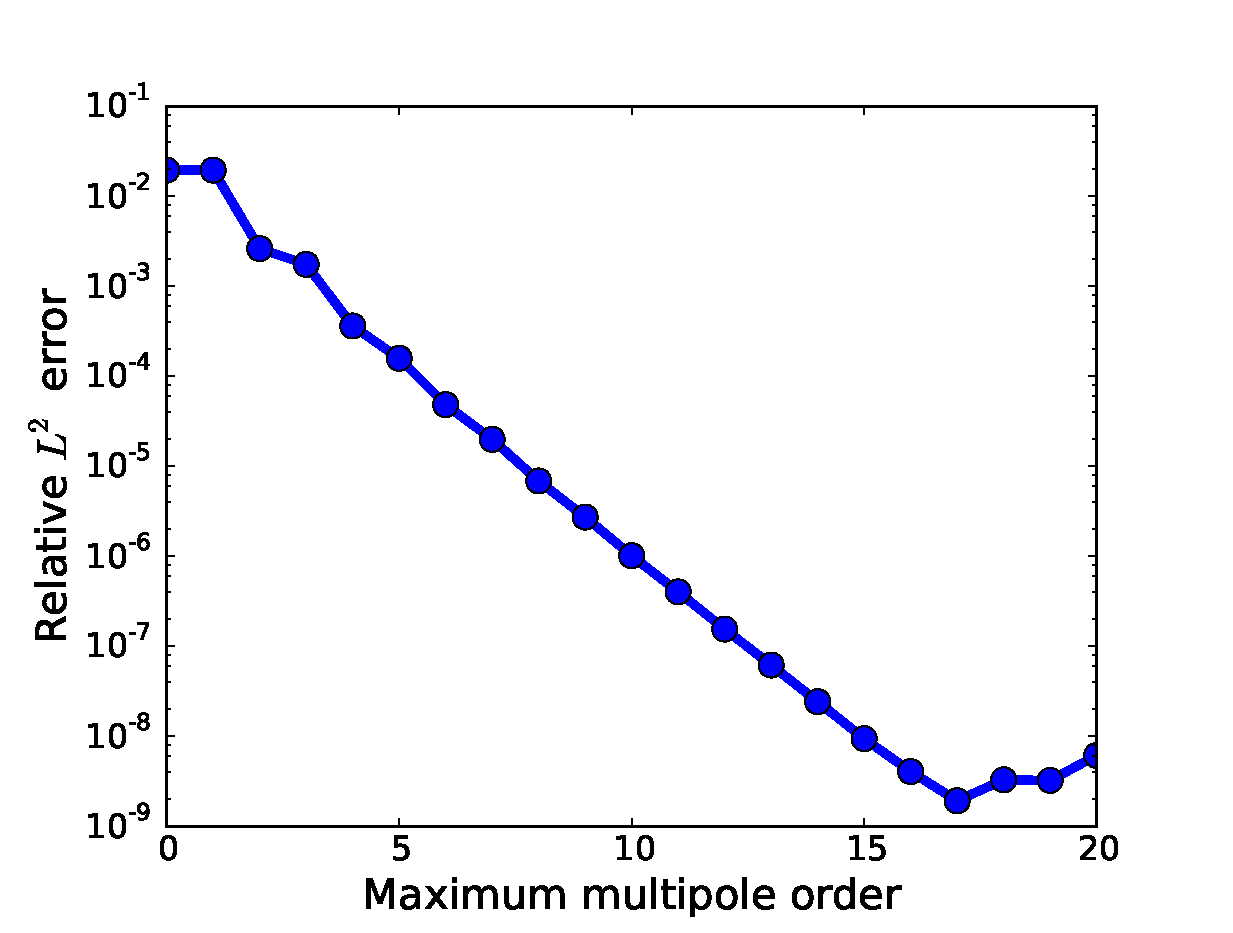
\includegraphics[scale=0.45]{plots/bc_comparison}
  \caption{Error of $\Phi$ on the computational domain for a binary white dwarf simulation 
    whose boundary conditions were computed using various values of the maximum multipole order,
    relative to the exact solution determined by a brute force sum on the boundaries.
    Circles represent the error at integer values, and they have been connected by a smooth 
    line to guide the eye.\label{fig:bc_comparison}}
\end{figure}


\subsubsection{Convergence Testing}\label{sec:gravity_convergence_testing}

Since the results of a merger simulation depend strongly on gravity,
it is important to check whether proper numerical convergence is
achieved for the Poisson solver. To do so, we created a simple test
that inserts a sphere of radius $R$ and uniform mass density $\rho$
onto our grid, and used \castro\ to calculate the gravitational
potential $\Phi$ of this setup. We ensure that $R$ is an integer
multiple of the grid spacing, and the center of the sphere is at the
origin. The problem domain for our simulations is $[-1.6, 1.6]^3$, and
we take $R = 1.0 \text{cm}$ and $\rho = 10^3\ \text{g cm}^{-3}$. 
The zones with $r > R$ are filled with an ambient material of very low density 
$\rho = 10^{-8}\ \text{g cm}^{-3}$. We run this problem at multiple 
resolutions corresponding to jumps by a factor of two. For
comparison, at each grid point we evaluate the analytical potential of
a uniform sphere, which can be easily determined using Gauss' law:
\begin{equation}
  \Phi_{\text{sphere}}(r) = -\frac{GM}{r} \times \begin{cases} (3R^2 - r^2)/(2 r^2) & r \leq R \\ 1 & r > R \end{cases},\label{eq:sphere-analytical}
\end{equation}
where $M = 4\pi R^3 / 3$ is the mass of the sphere. We measure the 
numerical error by calculating the $L^2$ norm of the error and 
normalizing it by the $L^2$ norm of the analytical solution:
\begin{equation}
  \text{Error} = \frac{\|\Phi - \Phi_{\text{sphere}}\|_2}{\|\Phi_{\text{sphere}}\|_2}.
\end{equation}
We define the order of convergence $p$ between two simulations with a jump 
in resolution of integer factor $m > 1$ as
\begin{equation}
  p = \text{log}_{m}\left(\frac{\text{Error}_{\text{low}}}{\text{Error}_{\text{high}}}\right).
\end{equation}
Here $\text{Error}_{\text{low}}$ is the $L^2$ error at the lower resolution 
and $\text{Error}_{\text{high}}$ is the $L^2$ error at the higher resolution.
We expect the error to converge at $p = 2$ given the discretization we choose. 
For all simulations in this section and for all our main science simulations,
we choose a relative error tolerance of $10^{-10}$ to be satisfied in the multigrid solve.
\begin{figure}[h]
  \centering
  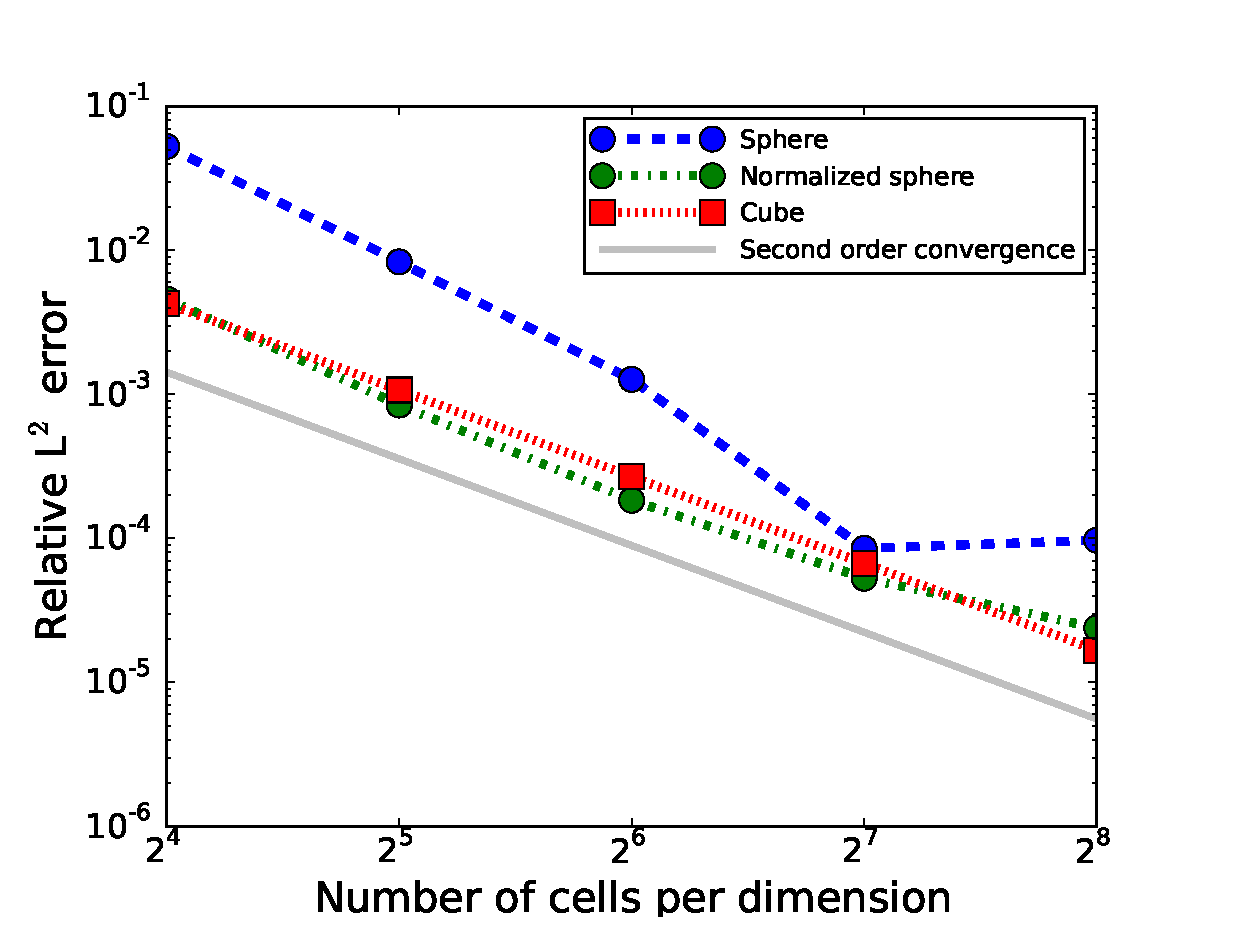
\includegraphics[scale=0.45]{plots/phi_comparison}
  \caption{Comparison of the \castro\ gravitational potential to the analytical solution for: 
    a sphere of uniform density; the same sphere, but with the potential normalized using the 
    actual amount of mass on the grid instead of the mass of a perfect sphere; and, a 
    cube of uniform density. Plotted also is a notional curve whose slope represents
    perfect second order convergence.\label{fig:gravity_convergence}}
\end{figure}
The results of this test are plotted in \autoref{fig:gravity_convergence}. 

We find that at low resolution 
convergence is actually substantially better than second-order. The 
explanation for this is that we are attempting to model a spherical 
object on a rectangular grid. At very low resolution, the object does 
not look very spherical. As the resolution is increased, the total 
amount of mass on the grid, as well as its location, will change 
as the sphere fills out. This means we are combining the true accuracy 
bonus from increased resolution with the artificial accuracy bonus 
from getting closer to solving the problem we are supposed to be solving. 
On the other hand, at the highest resolution shown the error slightly increases.

We can solve one of these two sources of error by evaluating 
\autoref{eq:sphere-analytical} with a mass $M$ that corresponds to the
amount of mass actually on the grid, defined as the sum of the density
multiplied by the volume of each cell for all cells whose density is 
greater than ambient. The resolution study for this case is also
plotted in \autoref{fig:gravity_convergence}. We still obtain
convergence slightly better than second-order, indicating that we 
still have the geometrical problem of the mass distribution changing.

The only way to fully eliminate this effect is to use a test problem that
does not change with resolution. The obvious companion is a cube of
uniform density $\rho$, where now $R$ is half of the side length of
the cube. At each resolution we use the same $R$ as for the sphere,
which ensures that the cube always fills exactly the same fraction of
the domain and thus has the same mass, so the only improvement comes
from better sampling at higher resolution. The gravitational potential for this
object has been worked out analytically by \citet{waldvogel:1976} (see
also a similar result by \citet{hummer:1996}, and an earlier calculation 
by \citet{macmillan:1958}). The potential is in
Equation 15 of that paper, though the last term is missing a factor of
$1/2$, which destroys the symmetry. Inserting this missing factor and
performing a simple coordinate transformation so that the center of
the cube is at the origin, the potential is
\begin{align}
  \Phi_{\text{cube}}(x,y,z) &= -G\rho\sum_{i,j,k=0}^1\left[x_i y_j\, \text{tanh}^{-1}\left(\frac{z_k}{r_{ijk}}\right)\right. \notag \\
  &+ \left. y_j z_k\, \text{tanh}^{-1}\left(\frac{x_i}{r_{ijk}}\right) + z_k x_i\, \text{tanh}^{-1}\left(\frac{y_j}{r_{ijk}}\right) \right.\notag \\
  &\left. - \frac{x_i^2}{2}\,\text{tan}^{-1}\left(\frac{y_j z_k}{x_i r_{ijk}}\right) - \frac{y_j^2}{2}\,\text{tan}^{-1}\left(\frac{z_k x_i}{y_j r_{ijk}}\right) \right. \notag \\
  &- \left. \frac{z_k^2}{2}\,\text{tan}^{-1}\left(\frac{x_i y_j}{z_k r_{ijk}}\right)\right]
\end{align}
where $x_0 = R + x$, $x_1 = R - x$, $y_0 = R + y$, 
$y_1 = R - y$, $z_0 = R + z$, $z_1 = R - z$, 
and $r_{ijk} = \sqrt{x_i^2 + y_j^2 + z_k^2}$. In
\texttt{Fortran} and \texttt{C}, the inverse hyperbolic tangent is
\texttt{atanh} and the inverse tangent is \texttt{atan} (\textit{not}
\texttt{atan2}). This formula is valid both inside and outside the
cube. The normalized $L^2$ error for this problem is also shown
in \autoref{fig:gravity_convergence}, and only for this problem 
do we obtain perfect second-order scaling at all resolutions.

The main lesson here is that in a convergence study, it is important
to ensure that the physical problem does not change with
resolution. Since in the case of spherical objects on rectangular
grids the effect may be to artificially boost convergence with resolution,
in a simulation with spherical objects like stars one can envision a
scenario of being fooled into believing apparently good convergence
results that are simply a convolution of artificially high
gravitational convergence and poor convergence in the hydrodynamics. A
convergence study in this case is only fully valid if there is reason
to be confident that this effect is negligible compared to other
factors.

\subsection{Rotation}\label{sec:rotation}

For the evolution of binary systems, it is most natural to evolve the
two stars in a frame that is co-rotating at the same period as the
orbital period. Since the publication of the original code paper, \castro\ 
now has the ability to evolve systems in a rotating reference frame. 
Source terms corresponding to the Coriolis and centrifugal 
force terms are added to the momentum and energy equations. In this frame, 
the stars essentially remain stationary in their original positions due to the
centrifugal force supporting against the gravitational attraction, and
will remain this way as long as significant mass transfer does not
occur. \cite{swc:2000} demonstrated (in the context of neutron star
mergers) that conservation of angular momentum is much easier to
obtain in the rotating reference frame than in an inertial frame in
which stars advect large amounts of material around the domain. We
wish to emphasize that although it is commonly stated in the
literature that grid-based codes poorly conserve angular momentum,
it is only generally true that grid-based codes do not exactly conserve 
angular momentum when the equations are written in conservative form
for linear momentum. (See also \cite{motl:2002} for an example of how 
to evolve the hydrodynamics equations for angular momentum.) 
The extent to which angular momentum conservation is violated
will be a function of the resolution. When this is sufficiently high
and a rotating reference frame is employed, excellent conservation
properties can result, as demonstrated in \autoref{sec:kepler}. 
In particular, at reasonable resolution for a binary orbit our code 
conserves angular momentum well enough that this no longer becomes 
a reason to use a Lagrangian method such as smoothed-particle hydrodynamics.
We note that as the stars begin to coalesce, the rotating reference frame
will no longer provide a good approximation to the spatial motion of
the stars and then they will begin to significantly move around the
domain. This is not necessarily problematic because the most important
feature of the rotating frame is that it helps ensure that the initial
coalescence is not the result of spurious numerical loss of angular
momentum. When significant mass transfer sets in and evolution
proceeds on a dynamical timescale, the conservation properties may be
slightly worse but angular momentum conservation is also less
important.

In a rotating reference frame with angular frequency vector $\bm{\omega}$, the momentum equation becomes:
\begin{equation}
  \left.\frac{\partial(\rho \mathbf{u})}{\partial t}\right|_{\text{rot}} = -2\, {\bm\omega} \times (\rho\mathbf{u}) - \rho {\bm\omega} \times \left({\bm\omega} \times \mathbf{r}\right).
\end{equation}
Here $\mathbf{r}$ is the position vector with respect to the origin. Typically we choose $\bm{\omega} = (0, 0, 2\pi / T)^T$,
with the rotation axis coincident with the $z$ axis at $x = y = 0$.
$T$ is the rotation period, which is the most natural quantity to specify
for a rotating stellar system. As described in the appendix, we include this source term
in the edge state prediction in a way that is analogous to the gravity source.
We evaluate all quantities at cell centers. We use the same predictor-corrector 
approach that we use for the gravity source terms to the momentum equations. However, a slight 
difference is that the Coriolis force for each velocity component is coupled to other velocity 
components. If the rotation is about the $z$-axis, then the discrete update to 
$v_x^{n+1}$ depends on the value of $v_y^{n+1}$, and vice versa. If we fix the value of 
the time-level $n+1$ quantities after coming out of the hydrodynamics update, there 
would be a slight inconsistency between the $x$ and $y$ components of the velocity. 

We propose a more accurate coupling that directly solves this implicit system of coupled 
equations. We denote by $(\widetilde{\rho \mathbf{u}})$ the value of the momentum after 
updating it with the centrifugal force, and the time-level $n$ Coriolis force. The remaining 
update for the time-level $n+1$ Coriolis force then appears as:
\begin{equation}
  (\rho \mathbf{u})^{n+1} = (\widetilde{\rho\mathbf{u}}) + \frac{\Delta t}{2} \left(-2\, {\bm\omega} \times (\rho\mathbf{u})^{n+1}\right)
\end{equation}
To proceed further, we assume that the rotation is about the $z$ axis with frequency $\omega$. 
Then there is no update to the $z$-momentum, and the other equations are:
\begin{align}
  (\rho u)^{n+1} &= (\widetilde{\rho u}) + \omega \Delta t (\rho v)^{n+1} \\
  (\rho v)^{n+1} &= (\widetilde{\rho v}) - \omega \Delta t (\rho u)^{n+1}
\end{align} 
We can directly solve this coupled system:
\begin{align}
  (\rho u)^{n+1} &= \frac{ (\widetilde{\rho u}) + \omega \Delta t (\widetilde{\rho v})}{1 + \omega^2 \Delta t^2} \\
  (\rho v)^{n+1} &= \frac{ (\widetilde{\rho v}) - \omega \Delta t (\widetilde{\rho u})}{1 + \omega^2 \Delta t^2}
\end{align}
We use this form of the momentum update in \castro. This improvement is small
but increases the accuracy of our rotating white dwarf systems over long time-scales.

The update to the energy equation can be determined by taking the dot product of the velocity
with the momentum source terms. The Coriolis term vanishes identically, and so
the Coriolis term does no work on the fluid. The update from the centrifugal force becomes
\begin{equation}
  \left.\frac{\partial(\rho E)}{\partial t}\right|_{\text{rot}} = \frac{1}{\Delta V}\int \rho \mathbf{u} \cdot \mathbf{f}^R\, dV,
\end{equation}
with $\mathbf{f}^R \equiv  -{\bm\omega} \times \left({\bm\omega} \times \mathbf{r}\right)$. 
This expression is identical in form to the gravity source under the interchange of $\mathbf{g}$ with $\mathbf{f}^R$.
As observed by \cite{marcello:2012}, we can similarly write down a rotational potential,
\begin{equation}
  \Phi^R = -\frac{1}{2} \left| {\bm\omega} \times \mathbf{r} \right|^2.
\end{equation}
So in the presence of rotation the total energy takes the form:
\begin{equation}
  (\rho E_{\text{tot}}) = (\rho E) + \frac{1}{2} \rho \Phi + \rho \Phi^R.
\end{equation}
Given that we can write down a potential energy for the rotation field, then we can use the machinery of 
\autoref{sec:gravity_hydro_coupling}. We again continue to evolve explicitly an equation for 
the gas energy, and allow it to change in response to work done by or on the rotational potential.
\begin{align}
  \left.\Delta(\rho E)\right|_{\text{rot}} &= - \sum_{f} \Delta \rho_{f} (\Phi^R_{f+1/2} - \Phi^R_{f-1/2})
\end{align}
Again we observe that this results a change in the global integral of $(\rho E)$, but keeps 
the global integral of $(\rho E_{\text{tot}})$ conserved (except at physical domain boundaries).

We apply the rotation forces after the gravitation forces, but 
there is some freedom in the order in which to apply the gravitational and rotational terms.
This order may matter because the Coriolis force depends on the fluid velocity, and 
in the predictor-corrector approach, we use the velocities both at 
time-level $n$ and time-level $n+1$. If we update the latter with the gravitational force, 
then the Coriolis force will see a different velocity than the one obtained through the 
pure hydrodynamics step. (This does not matter for the energy equation in our new formulation,
because the velocities used are always the time-level $n+1/2$ values coming from the Riemann solver.)
In practice, this will not matter significantly for our simulations in this work 
because the centrifugal force plays the dominant role in maintaining stability of non-contact 
binary systems, and the centrifugal force does not depend on the fluid velocity.
However, this issue may be worth exploring in future work in situations where the Coriolis 
term is non-negligible in determining the system evolution.

In all simulations performed in a rotating reference frame, we will transform all relevant
quantities back to the inertial reference frame when reporting them in this paper. In particular,
for every zone we add to the displayed kinetic energy the rotational energy associated with motion 
at the circular velocity corresponding to the distance of that zone from the rotation axis.
We do the analogous calculation for angular momentum as well. When plotting the locations of 
stars on the grid, we rotate them by an angle corresponding to the amount of time that has 
passed since the simulation started.

%==========================================================================
% Initial Models and Problem Setup
%==========================================================================

\section{Initial Models and Problem Setup}
\label{sec:initial_models}

At the start of any full simulation, we generate initial model white
dwarfs by integrating the equation of hydrostatic equilibrium, taking
the temperature and composition to be constant, and using the general
stellar equation of state.  This results in a single non-linear
equation to find the density in a zone given the conditions in the
zone beneath it:
\begin{equation}
\frac{p_{i+1} - p_i}{\Delta x} = \frac{1}{2} (\rho_i + \rho_{i+1}) g_{i+1/2}.
\end{equation}
This equation is a function of $\rho_{i+1}$ only since the pressure is
uniquely determined by the density in this case. Here, $\rho_i$ and $p_i$
are known, $g_{i+1/2}$ is the gravitational acceleration at the
interface between zones $i$ and $i+1$, found by simply adding up all
the mass from zones $1, \ldots, i$ to get the enclosed mass,
$M_{i+1/2}$, and then setting $g_{i+1/2} =
-GM_{i+1/2}/r_{i+1/2}^2$. We solve this equation for $\rho_{i+1}$
using a Newton-Raphson iteration.

We desire to specify the mass of the white dwarf, as well as its
temperature and composition. To start the integration off, we
therefore need to guess at a central density.  We then do a secant
iteration over the entire integration procedure to find the central
density needed to yield the desired total mass.  The grid spacing is
$\Delta x = 6.25\ \text{km}$. We chose this value because no simulation
we perform is likely to exceed this grid resolution inside the stars 
themselves; for our normal domain size (see below), this corresponds to 
three jumps in refinement by a factor of four. We find that for low 
resolution runs, this is a better choice than selecting the 1D grid 
spacing to be equal to the 3D grid spacing.

We map the 1D model onto the 3D Cartesian grid by taking density,
temperature, and composition as the independent variables,
interpolating these to the cell centers, and then calling the equation
of state to initialize the remaining terms. It is possible to interpolate
instead by using pressure instead of temperature, as pressure is more 
closely related to hydrostatic balance, but the EOS we use is so 
insensitive to temperature that this mapping can result in large 
deviations from the isothermal assumption we started with.  The 
interpolation process divides each zone into $n_{\text{sub}}$ 
sub-zones of equal volume for
the purpose of sampling the 1D model, and the sub-zones are added
together to obtain the full zone's characteristics. This
sub-grid-scale interpolation is useful especially near the edge of the star,
where the density falls off rapidly with radius. Typically we take 
$n_{\text{sub}} = 4$.

For a single star simulation, the star is simply placed at the center
of the computational domain, which we take to be the origin. For a
binary star simulation, we take as parameters the mass of the two
white dwarfs and the initial orbital period $T$. Using Kepler's third
law and assuming a circular orbit, we can then work out the orbital
separation $a$:
\begin{equation}
  a = \left(\frac{GM T^2}{4\pi^2}\right)^{1/3}.
\end{equation}
Here $M = M_P + M_S$ is the total mass of the system, where $M_P$ is
the specified \textit{primary} mass and $M_S$ is the specified
\textit{secondary} mass. The primary WD will always start on the left
side of the computational domain for our simulations, and is more
massive than the secondary. This reflects the usual terminology in the
literature where the primary WD is the accretor and the secondary is
the donor. The center of mass is located at the center of the
computational domain, and the stars lie along the $x$ axis, so that
the primary's center of mass is located at $x = -(M_S / M)\, a$ and
the secondary's center of mass is located at $x = (M_P / M)\, a$.

The initial velocity is taken to be zero in if we are in the reference
frame that rotates with the WDs, and if we are in the inertial frame
the velocity in every zone is set equal to the rigid rotation rate 
corresponding to the distance of that zone from the rotation axis, given
the specified period $T$. Thus the inertial frame and rotating frame 
simulations are starting off with the same initial conditions: two white 
dwarfs locked in synchronous rotation. This is the simplest assumption to 
make, but in the future we may explore relaxing this requirement.

We do not attempt to enforce equilibrium with an additional relaxation
step. This will be an important part of future work in this series, as
numerous groups working on binary evolution
\citep{swc:2000,motl:2002,rosswog:2004,dan:2011,pakmor:2012:gadget}
have commented on the importance of equilibrium initial conditions in
determining the evolution of the system. As a consequence of starting 
in a non-equilibrium setting, there are 
large density and pressure gradients near the white dwarf surfaces
that result in large amounts of mass flowing into the ambient
medium. This can result in spurious non-physical consequences such as 
the total density or energy going negative in a zone. To compensate 
for this, we start the simulation with a timestep that is a few orders 
of magnitude smaller than that required by the CFL criterion, and allow
the timestep to increase by 1\% each timestep so that the timestep reaches 
its maximum allowed by the velocities on the grid over a span of approximately 
1000 timesteps. This allows the ambient medium just outside the white dwarf
to come closer to equilibrium with the surface without having 
discontinuous jumps in the density or energy. For all simulations, 
the maximum timestep is set to be equal to one-half of the CFL limit.

We track a number of diagnostic quantities at the end of every coarse grid timestep. 
For all simulations, we record the total energy (including the breakdown into
its components: kinetic, internal, gravitational potential, rotation; we note
that for the diagnostics we actually use $(\rho E)$ for calculation of the total energy,
rather than explicitly calculating the sum of kinetic and internal, as this is
the quantity that should be explicitly conserved), 
the total angular momentum, and the center of mass of the system. 
For stellar calculations, we separately record diagnostic 
information about the stars. Our strategy for tracking their 
locations is as follows: at the beginning of the calculation, we store the 
physical center of mass $\mathbf{x}_{\text{COM}}$ of the stars as determined 
by Kepler's third law. We also store the space velocity $\mathbf{v}_{\text{COM}}$ 
of the stars. Then, at each new time step we make a preliminary guess for their 
location by updating the location using the old velocity, 
$\mathbf{x}_{\text{COM}} \rightarrow \mathbf{x}_{\text{COM}} + \mathbf{v}_{\text{COM}} \Delta t$.
We then refine our guess for the location and velocity of each star by computing a
location-weighted sum of the mass and velocity over the computational domain. 
To do this, we need a cutoff for determining what counts as part of the primary 
and what counts as part of the secondary. For this we can use the formula provided by 
\citet{eggleton:1983} for the effective Roche radius $r_L$ of a star in a binary,
\begin{equation}
  \frac{r_L}{a} = \frac{0.49 q^{2/3}}{0.6^{2/3} + \text{ln}(1 + q^{1/3})}.
\end{equation}
In this formula we can use $q = M_S / M_P$ for obtaining the Roche radius of the secondary,
and use the inverse value of $q$ to obtain the Roche radius of the primary.
To a reasonable approximation, all material within the effective Roche radius
of each star can be counted as belonging to that star. From this we obtain the mass
of each star as well as its location and velocity. Once we have the new centers of mass,
we compute the effective radius of each star at various density cutoffs. This involves 
computing the volume $V$ of all zones within the Roche radius of the star's center 
whose density is greater than the cutoff. We then compute $r_{\text{eff}} = (3V/4\pi)^{1/3}.$

A final diagnostic quantity we consider is the gravitational wave emission by the 
binary system. White dwarfs are not strongly affected by general relativistic effects;
the orbital motions are much slower than the speed of light, and the relativity parameter 
$GM / c^2 R$, which measures the ratio of the Schwarzschild radius of a mass $M$ to the actual 
radius $R$ of the object, is much less than unity for a white dwarf. It is justified to 
neglect any relativistic effects in computing the dynamical evolution of the system. However,
the system emits gravitational waves during its evolution; this energy loss is what drives 
the initial inspiral over very long timescales, and occurs at a greater rate during 
the coalescence phase, though then being inconsequential on a dynamical timescale. The 
frequency of the gravitational waves will be similar in size to the frequency of the 
orbital motion, which is in the range 10-100 mHz for our problem. This is well outside 
the range of currently existing gravitational wave detectors but is very well suited 
for proposed space-based detectors such as eLISA.

We follow the prescription of \citet{blanchet:1990}. At distances far from the 
gravitational wave source, we can consider the leading term in the gravitational 
wave signal:
\begin{equation}
  h^{TT}_{ij}(t,\mathbf{x}) = \frac{2G}{c^4 r}P_{ijkl}(\mathbf{n}) \ddot{Q}_{kl}(t - r/c).
\end{equation}
$h$ is the perturbation to the spacetime metric and is commonly called the \textit{strain}; 
for laser interferometers, it measures the relative change in the distance between mirrors. 
The ``TT'' superscript indicates that we work in the commonly used tranverse-traceless gauge.
This strain is measured at time $t$ and position $\mathbf{x}$ relative to the binary system.
$r\equiv |\mathbf{x}|$ is the distance from the observer to the binary system. The unit vector 
$\mathbf{n} \equiv \mathbf{x} / r$ then measures the direction of the outgoing wave with 
respect to the observer, and $P_{ikjl}(\mathbf{n})$ is an operator in the transverse-traceless 
gauge that projects a tensor onto the direction orthogonal to $\mathbf{n}$:
\begin{align}
  P_{ijkl}(\mathbf{n}) &= \left(\delta_{ik} - n_i n_k\right)\left(\delta_{jl} - n_j n_l\right) \notag \\
                      &- \frac{1}{2}\left(\delta_{ij} - n_i n_j\right)\left( \delta_{kl} - n_k n_l\right).
\end{align}
$Q_{kl}$ is the quadrupole moment tensor:
\begin{equation}
  Q_{kl} = \int dV \rho \left(x^k x^l - \frac{1}{3}\delta^{kl} \mathbf{x}^2\right).
\end{equation}
The argument $(t - r/c)$ indicates that to get the strain at time $t$ we evaluate the second derivative of the 
quadrupole moment at the retarded time $t - r/c$. In practice we ignore this in calculating this strain,
instead using the current simulation time, and so this merely yields a time delay of order $r/c$ between 
when the waves are emitted and when we observe them. 

Therefore the primary component of the calculation is the evaluation of the second time derivative of $Q_{kl}$.
Explicitly constructing a discretized form of this derivative, using the current state and the state at 
previous times, is undesirable because of the inherent imprecision (its accuracy depends on the size of the timestep),
in addition to the logistical challenges that may be implied by saving and using previous simulation states. 
\citet{blanchet:1990} provide a prescription for this time derivative purely in terms of the state at a given time:
\begin{equation}
  \ddot{Q}_{kl} = \text{STF}\left\{2\int dV \rho (v^k v^l + x^k g^l)\right\}.
\end{equation}
The symmetric trace-free (STF) operator is defined as:
\begin{equation}
  \text{STF}\left\{A^{ij}\right\} = \frac{1}{2}A^{ij} + \frac{1}{2}A^{ji} - \frac{1}{3} \delta^{ij} \sum_{k}A^{kk}.
\end{equation}

The strategy is then as follows. At the end of the coarse timestep, we first calculate $\ddot{Q}_{kl}$
using an integral over the domain (using refined grids as usual by masking out the contributions from 
coarse grids underlying more accurate fine grids). This quantity is independent of the observer. If we 
are using a rotating reference frame, we first convert velocities and positions back to the inertial 
frame before evaluating the integral. Then, 
we pick an observing location $\mathbf{x}$ relative to the domain, evaluate the projection operator, 
and then perform the relevant tensor contraction to determine the strain tensor. We can 
repeat this process for any number of observing locations at minimal cost, since the quadruple tensor 
only needs to be calculated once. Now, gravitational waves only excite modes orthogonal to their 
direction of travel. These are the ``plus'' and ``cross'' modes, $h_+$ and $h_\times$, named after 
the types of spatial distortions they exhibit. We calculate the signal at a distance $r$ along 
the $x$, $y$ and $z$ axes. For the latter, as an example, $h_{+} = h_{11} = -h_{22} \propto (\ddot{Q}_{11} - \ddot{Q}_{22})/2$ and 
$h_{\times} = h_{12} = h_{21} \propto \ddot{Q}_{12}$. All other entries vanish. By default we take $r = 10$ kpc; 
as shown by \citet{loren-aguilar:2005}, this is a typical distance scale over which an 
experiment such as LISA could detect a coalescing binary white dwarf system. 
However, the strain at any other distance is easily calculated and goes as the inverse of the distance.

The computational domain has a total size of $1.024 \times 10^{10}\ \text{cm}$ in each 
spatial dimension, and is centered at the origin. Our coarse grid has $256^3$ zones,
corresponding to a spatial resolution of 400 km. For the present study, we choose a simple 
refinement strategy: all zones within twice the Roche radius of each star are tagged for maximal 
refinement. The extra buffer from doubling the size of this region ensures that the sharp density
gradients near the edge of the star are within the zone of refinement. We also ensure that the 
outer part of the domain is never tagged for refinement. In future work we will add criteria 
that tag for refinement the gas between the stars, which is expected to feature nuclear burning.

For ghost cells at the physical edge of the domain, we always use quantities 
corresponding to the initial ambient material, to prevent material from raining down
on to the grid in response to the disequilibrium outside the stars. This is an artificial 
choice, but the dynamics outside of the stellar orbit is arbitrary anyway, due to the 
lack of knowledge about the density and velocity field inside this gas. In addition, we employ 
a ``sponge'' similar to that described by \citet{maestro3}. After the hydrodynamics update (but before 
the gravity and rotation correction terms), we apply a damping force to the momentum 
equation as follows:
\begin{equation}
  (\rho \mathbf{u})^{n+1} \to \frac{(\rho \mathbf{u}^{n+1})}{1 + (\Delta t / \Delta t_S) f_S},
\end{equation} 
where $\Delta t_S$ is a timescale for the sponge to operate on, and $f_S$ is the damping factor.
We choose it so that that the sponge is non-operational inside a radius $r_S$ from the origin, and 
fully applied at a radius $r_S^\prime \equiv r_S + \Delta r_S$. We then smooth the sponge 
out between $r_S$ and $r_S^\prime$:
\begin{equation}
  f_{S} = \begin{dcases} 0 & r < r_S \\ \frac{1}{2}\left(1 - \text{cos}\left[\pi\left(\dfrac{r - r_S}{\Delta r_S}\right)\right]\right) & r_S \leq r < r_S^\prime \\ 1 & r \geq r_S^\prime. \end{dcases}
\end{equation}
For the simulations in this paper we set $r_S$ to be 75\% of the distance from the origin to the domain boundaries,
and $\Delta r_S$ so that the sponge extends another 10\% of that distance. We set 
$\Delta t_S = 0.01$ s, which is of the same order as the as the CFL timestep 
for typical problem setups. We find that this sponge is necessary especially in the 
rotating reference frame, as standing instabilities can create very large velocities 
in the ambient fluid that drag down the global timestep by up to an order of magnitude.
However, this provides another reason to distrust the dynamics of the low-density fluid
outside of the stellar orbits.

The software used to generate the test problems in this paper
(as well as the manuscript itself),
\wdmerger\footnote{\wdmerger\ can be obtained at \url{https://github.com/BoxLib-Codes/wdmerger}.},
is freely available at an online repository hosting service.
Version control in both the parent software (\boxlib, \castro) and in \wdmerger\
permits us to reference the state of the code at the time a simulation
was performed. In all plot files and diagnostic output generated by \castro, 
and EPS figure files and plots generated by \wdmerger\ for this work,
we store the active \texttt{git} commit hashes of \boxlib, \castro, and \wdmerger.
Line plots are generated using the \matplotlib\ library for \python\ 
\citep{matplotlib}, while slice plots and other multi-dimensional visualizations are 
generated using the \yt\ code \citep{yt}.



%==========================================================================
% Numerical Test Problems
%==========================================================================
\section{Numerical Test Problems}\label{sec:Tests}

Merger simulations face a number of numerical difficulties that are
not present in single-degenerate Type Ia and core-collapse supernova
simulations. In \autoref{sec:gravity}, we discussed how the lack
of spherical symmetry necessitates a careful look at the gravity
solver. There are also hydrodynamical issues: the merger process will
result in substantial motion of stellar material across the grid. This
bulk motion presents an opportunity for advection errors to build up,
and is only partially mitigated by evolving the white dwarfs in a
co-rotating frame. It is therefore important to be be aware of the
behavior of the code in such circumstances. The behavior of \castro\ for
many standard hydrodynamics test problems was detailed in the original
code paper \citep{castro}, and in the interest of brevity we will not
repeat them here. Instead, we focus on a subset of problems that
highlight the special difficulties introduced in merger
simulations. These problems couple the hydrodynamics, gravity and
equation of state modules. We observe that while in most non-trivial
three-dimensional problems this creates a complexity that makes it
impossible to determine exact analytical solutions, it is
straightforward to devise problems for which certain global properties
should obey simple, expected behaviors. Where possible, these should
be quantified and a convergence study performed. We recommend that all
simulation codes should check their performance on such problems to
ensure their reliability when coupling the various physics modules
necessary to build a complete and realistic simulation.

\subsection{Maintaining Hydrostatic Equilibrium}\label{sec:HSE}

In \autoref{sec:initial_models} we describe the process by which
we generate initial stellar models. While the 1D models are in
hydrostatic equilibrium to within a small error, interpolation onto
the 3D Cartesian grid will introduce perturbations into the solution
\citep{zingale:2002}. Although we ensure that the initial models are
generated with the same equation of state and are as well resolved as
our finest grid, there will still be a hydrodynamical error associated
with the fact that the rectangular grid cannot faithfully represent a
spherical star. Additionally, the gravitational potential obtained by
the multigrid solver will differ slightly from the one assumed by the
initial model, and the operator splitting between the gravity and
hydrodynamics should also result in small errors. As a result, we
expect that the star will oscillate slightly about an equilibrium
point, but that the amplitude of this oscillation should decrease with
increasing resolution.

\begin{figure}
  \centering
  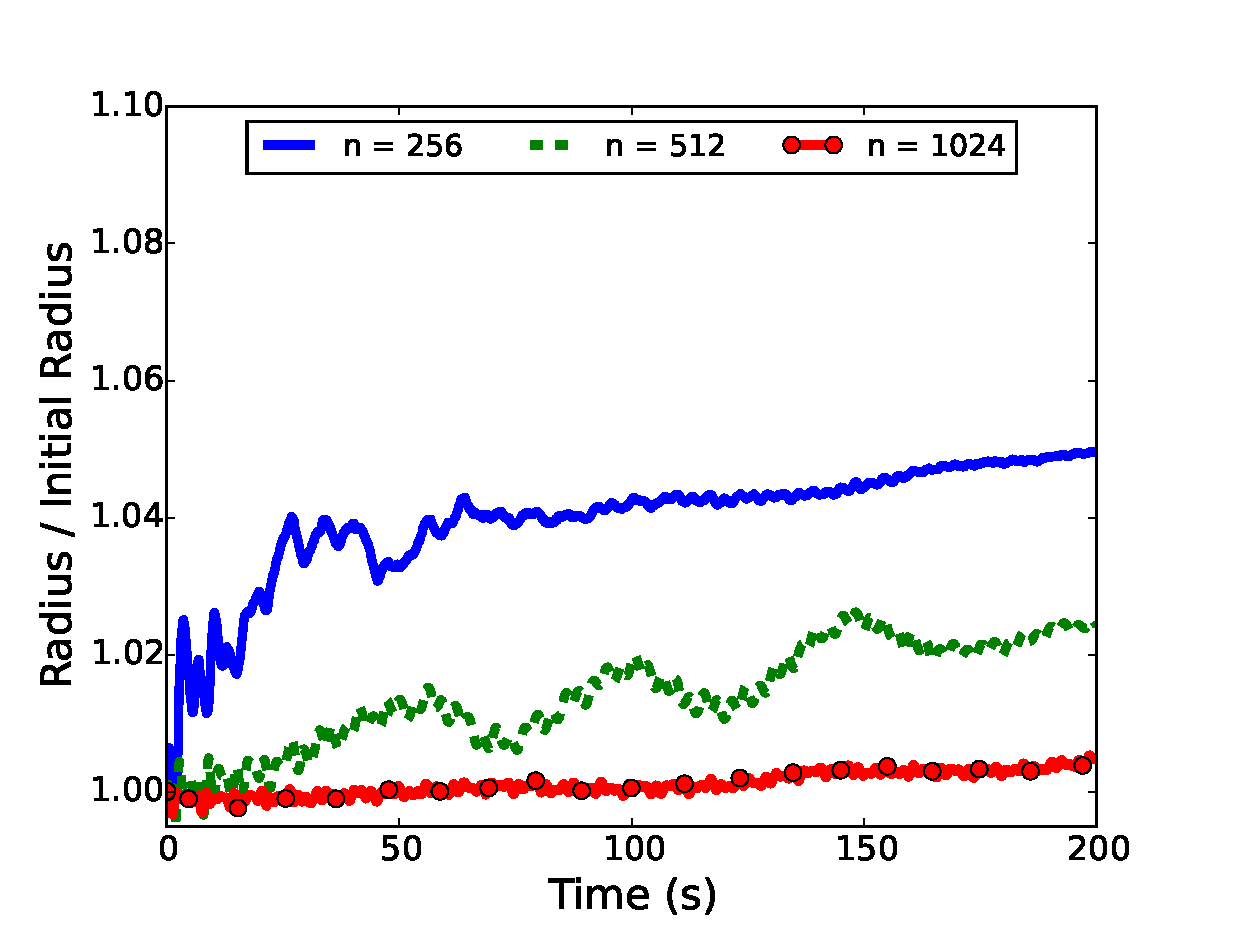
\includegraphics[scale=0.45]{plots/single_star_static_1e3_radius}
  \caption{Time evolution of the effective radius of a $0.9 \msolar$ 
    white dwarf, seeded onto the grid using a one-dimensional hydrostatic
    model and evolved without further relaxation. The lines represent 
    different number of zones per spatial dimension; when this number is 
    greater than 256, it represents an effective resolution obtained 
    using AMR levels that cover the star. The radius is determined 
    using the volume of the grid that has a density greater than $10^3\ \text{g cm}^{-3}.$
    \label{fig:single_star_static_radius}}
\end{figure}

This problem was studied in the first \castro\ paper, but is worth
revisiting here. A single star explosion simulation may only last a
couple of seconds, and the \castro\ paper studied the behavior of the
star after one second of evolution. However, the dynamical timescale
of a typical carbon-oxygen white dwarf is on the order of 1--10
seconds. Additionally, a binary orbit is typically on the order of
10--100 seconds when a merger simulation starts, and with equilibrium
initial conditions the system may survive for tens of orbits before
the secondary is disrupted. When this does happen, we want to be
confident that it was because of the dynamics of the merger process
and not because of an instability in an individual star. Our goal here
is thus to populate a single star onto our three-dimensional
coordinate grid and evolve it for a period of time long enough to
assess whether the star is truly stable, and to probe how the size of
deviation from equilibrium is affected by grid resolution.

We loaded a single star of mass $0.9\ \msolar$ onto the grid at the origin, 
and evolved it for 200 seconds. Our diagnostic of choice is the effective 
radius of the star, determined by the volume of the grid that has a density 
greater than $10^3\ \text{g cm}^{-3}$ (see \autoref{sec:initial_models} 
for details on this measure). This choice of density is intended to 
mark a reasonable outer edge to the star that is not immediately susceptible 
to the numerical errors prevalent near the physical edge of the star. 
\autoref{fig:single_star_static_radius} shows our results at various resolutions. 
As expected, the star quickly approaches an equilibrium size that is different 
(and in this case larger) than the one-dimensional model. However, the magnitude 
of this change becomes smaller with resolution. The star is only approximately 
in equilibrium Only when the coarse grid of $256^3$ zones has a level of 
refinement that jumps by a factor of four. However, even then there is a slight 
uptick in the size toward the event, implying that the numerical stability 
is not guaranteed for arbitrarily long timescales. This result suggests that when 
doing the equilibrium initial models that will former the basis of later calculations,
we should carefully monitor the evolution of the stars before applying any 
artificial damping to cause the merger, to ensure that the merger is due to 
this applied force and not the intrinsic numerical instability of the stars.

\begin{figure}
  \centering
  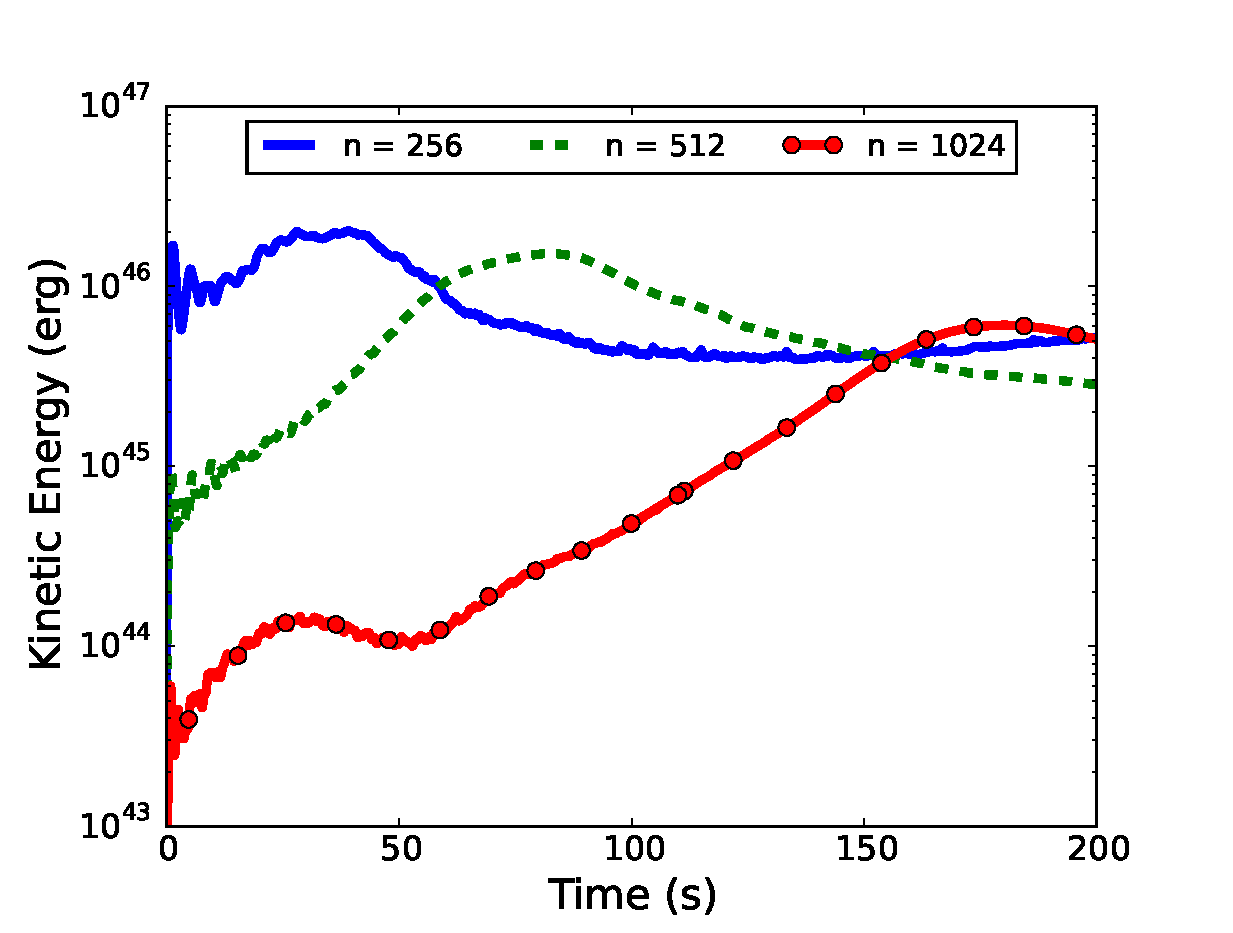
\includegraphics[scale=0.45]{plots/single_star_static_ke}
  \caption{Time evolution of the kinetic energy of a $0.9 \msolar$ 
    white dwarf. The lines have the same meaning as in \autoref{fig:single_star_static_radius}.
    \label{fig:single_star_static_ke}}
\end{figure}

\subsection{Gravitational Free Fall}\label{sec:Gravitational Free Fall}

A simple dynamical test to verify the gravitation physics in \castro\ is
the case of gravitational free fall. We place two stars on the grid 
in the manner of \autoref{sec:initial_models}. The distance $a$ between 
them corresponds to a chosen orbital period $T$, consistent with the total
system mass $M$, but we disable the rotational source terms so that 
the stars start at rest in an inertial reference frame. 
Thus the stars will simply begin moving toward each other.
As long as the stars remain approximately spherical, the stars can be 
treated as point masses (this only seriously breaks down after the stars
have come into contact). In dimensionless units where $r \to r / a$ and 
$t \to 2\sqrt{2}\pi t / T$, the simple free fall equation of motion governing the
distance $r$ between their centers of mass takes the form:
\begin{equation}
  \ddot{r}(t) = - \frac{1}{2r^2}.
\end{equation}
It is possible to derive a closed-form solution for the evolution time
as a function of separation by starting with the integral formulation,
\begin{equation}
  t(r) = \int_{1}^{r} \frac{dr}{v(r)}.
\end{equation}
The velocity $v$ (in dimensionless units) can be found by noting that 
$\ddot{r} = v\, dv / dr$ and then separating and integrating the equation 
of motion. This yields 
\begin{equation}
  v(r) = \sqrt{\left(\frac{1}{r} - 1\right)}.
\end{equation}
For our problem $0 \leq r \leq 1$, so this is always valid. Integrating, we find
\begin{equation}
  t(r) = \text{arccos}\left(\sqrt{r}\right) + \sqrt{r \left(1 - r\right)}. \label{analyticalFreeFall}
\end{equation}
so that the point of contact would occur at $t = 1$. We actually stop the simulation
at $t = 0.9$, which is when the effects from the extended sizes of the stars
starts to become important. The results of our simulation for our default $256^3$ zone 
uniform grid are shown in \autoref{fig:freefall}. They show excellent agreement
between the theory and the simulation results, and this agreement holds even for 
a more moderate $128^3$ zone simulation.

\begin{figure}
  \centering
  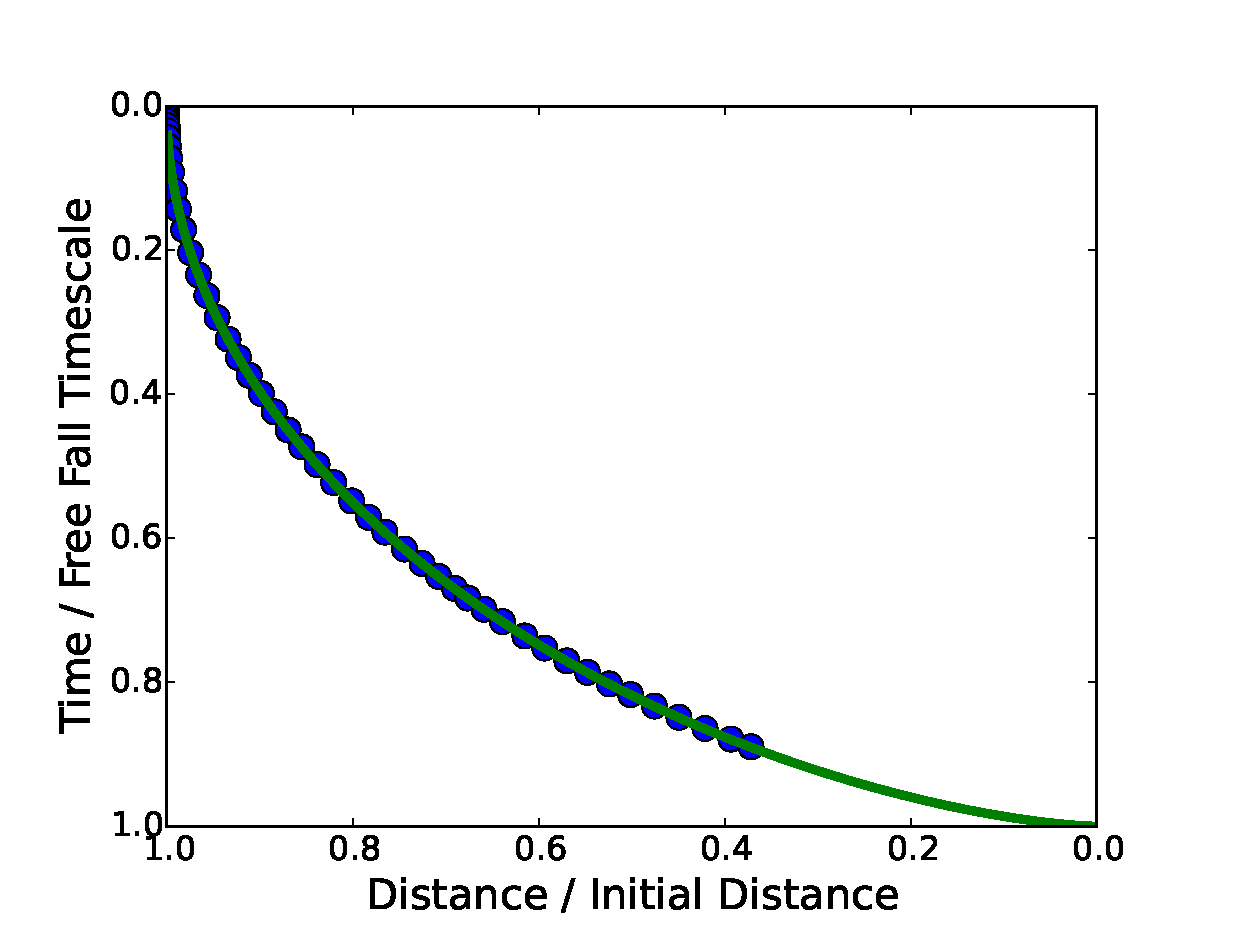
\includegraphics[scale=0.45]{plots/freefall}
  \caption{Time evolution of two initially stationary white dwarfs,
    mutually attracted to each other by the gravitational force. The
    horizontal axis gives the separation of the white dwarfs, scaled
    to the initial separation, and the vertical axis gives the elapsed
    time of the simulation, scaled to the time it would take two point masses
    to collide. The solid curve shows the analytical result,
    calculated from Newtonian mechanics, and the circles show the
    samples from the time evolution with \castro. For visual clarity, we 
    show only a small fraction of the timesteps.}
  \label{fig:freefall}
\end{figure}

\subsection{Galilean Invariance}\label{sec:galileo}

It is often stated in the literature that Eulerian methods for
hydrodynamics with grids fixed in space do not obey the Galilean
invariance of the underlying Euler equations, so that simulations
moving at a uniform bulk velocity will appear different than an
equivalent stationary simulation. If true, we need to understand 
the importance of this effect when deciding whether to trust the 
output of a code like \castro\ when applied for merger problems.
Recently, this has come up in two ways which are of note for us 
in the present study. We will explain these situations and display 
the results of tests we have run to determine whether this 
actually is a significant concern for our study.

\citet{arepo} (hereafter, S10) performed a Kelvin-Helmholtz instability test and showed
that (at low resolution) a fixed-grid code failed to develop the
expected fluid instability when the whole fluid was moving at a
strongly supersonic uniform velocity. (See also \citet{wadsley:2008}, 
who used the FLASH code to simulate a hot bubble subject to mixing 
by the Kelvin-Helmholtz instability, and also found that the mixing was affected by a 
uniform bulk velocity.) This contrasted with the results
of the moving-mesh code AREPO being presented in that study, which
demonstrated Galilean invariance even at large bulk velocities. 
Inability to correctly model the Kelvin-Helmholtz instability would 
ave important consequences for how much we can trust the ability of 
\castro\ to test the violent merger progenitor model. Shearing between 
the material flowing out of the secondary and material near the 
surface of the primary may trigger fluid
instabilities that play an important role in the evolution of that
gas, which is the site of the initial detonation in the prompt
explosion model. \citet{guillochon:2010} showed for their simulation
that Kelvin-Helmholtz instabilities produced this way may raise the
temperature of the accreting material enough to ignite a
detonation. Therefore if we are not correctly reproducing the
characteristics of the Kelvin-Helmholtz instability in the case where
there is significant mass motion on the grid, we cannot be confident
that a detonation (or lack thereof) is not numerically
seeded. 

\begin{figure*}[ht]
  % Note that since we have periods in the filename, we need to double-
  % bracket the filename so that includegraphics doesn't think it's 
  % looking for something with the wrong extension. See:
  % http://tex.stackexchange.com/a/10575
  \centering
  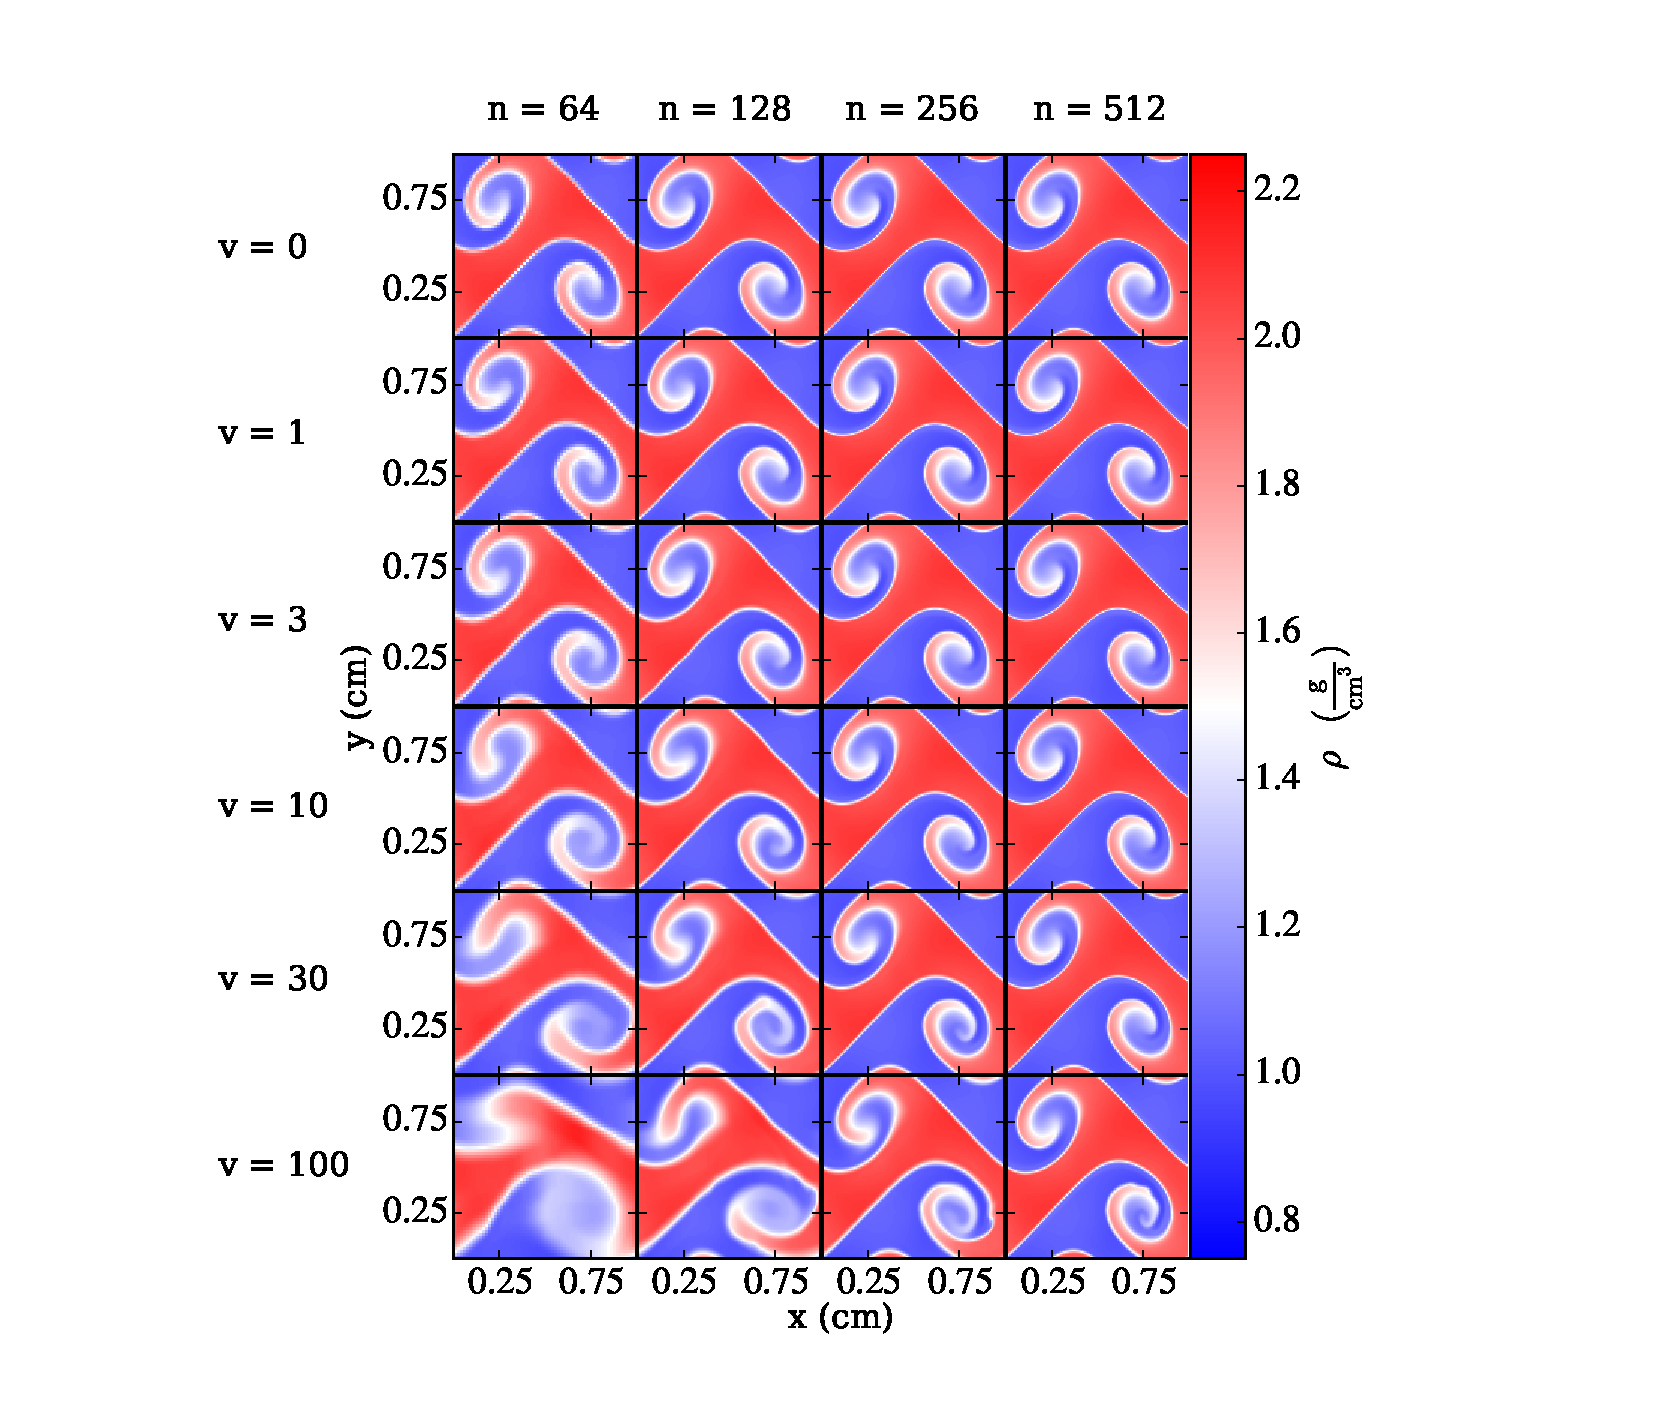
\includegraphics[trim=0.75in 0.45in 0.85in 0.5in, clip, scale = 0.75]{{{plots/kh_t2.0_p2_low_res_collage}}}
  \caption{2D Kelvin-Helmholtz instability test at $t = 2.0$ for the initial 
    conditions given by \autoref{eq:kh_ic_b_ramp} and \autoref{eq:kh_ic_b}. 
    The rows each represent a different bulk fluid velocity $v$ and 
    the columns each represent a grid resolution $n$ (the number of 
    zones per spatial dimension). The highest velocity simulation, 
    $v=100$, corresponds to approximately Mach 70. Compare to 
    Robertson et al. (2010), Figure 7. \label{fig:kh_p2}}
\end{figure*}

\citet{robertson:2010} (hereafter, R10) observe that Galilean
invariance of simulation results for the Euler equations occurs only
because of truncation error in the discretization of the fluid
equations. This takes the form of a numerical diffusion term which is
dependent on velocity (and also resolution). The advantage of a
moving-mesh code is that the mesh everywhere moves with the local flow
velocity, which substantially reduces the numerical
diffusion. R10 argue that the differences seen
between the moving-mesh and fixed-grid code are caused by the
interaction of this numerical diffusion with small-scale instabilities
(which may be physical or numerical) which couple with and
fundamentally alter the large-scale modes. Small-scale instabilities
are seeded by the choice of a sharp initial discontinuity between the 
fluids in the problem posed by S10. Crucially though,
R10 point out that this problem does not
converge with resolution and so it is not possible to know the correct
behavior of this problem. As such, we do not know whether the
small-scale modes found in AREPO are real, and the problem is not
useful in formally discriminating between methodologies. They instead
propose an alternate test with a smoother initial contact. This
converges to the same solution qualitatively in both the stationary
and bulk velocity cases, indicating that the code does generally
maintain Galilean invariance (to some specified error that depends on
resolution and the uniform flow speed).  We will see whether we can
reproduce this result.

A related question is whether our code reliably simulates the bulk
motion of the stars across the grid, and whether such bulk motion
affects the stability of the star. This concern is prompted by the
study of \cite{tasker:2008}, who studied the effect of uniform
translation on the stability of a spherically symmetric model for a
galaxy cluster. They compared the radial profile of the cluster at
initialization and after a period of time evolution. Using FLASH and
ENZO, they found that a static cluster retains its shape at high
enough resolution, while uniform translation of the cluster causes
mixing of the core material due to numerical diffusion which results
in an underestimation of the core's true density. The SPH codes they
used did a better job maintaining the core density. We will perform a
variant of this test using white dwarf models.

\subsubsection{Kelvin-Helmholtz Instability}\label{sec:khi}

Following \cite{robertson:2010}, we set up a Kelvin-Helmholtz test in
the following way. The problem domain runs from 0 to 1 in both the $x$
and $y$ directions. This is a two-dimensional test, so we run
\castro\ in 2D mainly to avoid extra computational expense; in 3D, it 
would merely involve replicating the problem in the $z$ direction.
The problem involves a fluid slab of density $\rho_2 = 2.0$ traveling rightward in the
$x$-direction at velocity $v_2 = 0.5$, sandwiched by a fluid of
density $\rho_1 = 1.0$ traveling leftward at velocity $v_1 =
-0.5$. The density gradient is in the $y$ direction, so this creates a
velocity shear along the interface between the fluids. The density and
velocity distribution on the computational domain are given by:

\begin{align}
  \rho &= \rho_1 + R(y)\left[\rho_2 - \rho_1\right] \\
  v_x  &= v_1 + R(y)\left[v_2 - v_1\right] \\
  v_y  &= v_{\text{bulk}} + v^\prime
\end{align}

Here $R(y)$ is a ramp function that describes the transition between
the two fluids, while $v_{\text{bulk}}$ is the bulk motion of the
fluid in the $y$ direction and $v^\prime$ is the velocity perturbation
that seeds the instability. The problem will be established for two
sets of initial conditions (ICs), which we follow
R10 in calling ICs A and B. They differ in
their ramp function ($R_A$ and $R_B$ respectively), as well as the
initial perturbation ($v^\prime_A$ and $v^\prime_B$ respectively), and
the frequency of the perturbation ($n_A = 4$ and $n_B = 2$):
\begin{align}
  R_A &= \begin{cases} 0 & |y - 0.5| > 0.25 \\ 1 & |y - 0.5| < 0.25 \end{cases} \label{eq:kh_ic_a_ramp}\\
  R_B &= \Big\{\left[1 + e^{-2(y-0.25)/\Delta_y}\right]\left[1 + e^{2(y-0.75)/\Delta_y}\right]\Big\}^{-1} \label{eq:kh_ic_b_ramp}\\
  v^\prime_A &= w_0\, \text{sin}\left(n_A\, \pi\, x\right) \left\{e^{-(y-0.25)^2 / 2\sigma^2} + e^{-(y-0.75)^2/2\sigma^2}\right\} \label{eq:kh_ic_a}\\
  v^\prime_B &= w_0\, \text{sin}\left(n_B\, \pi\, x\right). \label{eq:kh_ic_b}
\end{align}

\begin{figure*}[ht]
  \centering
  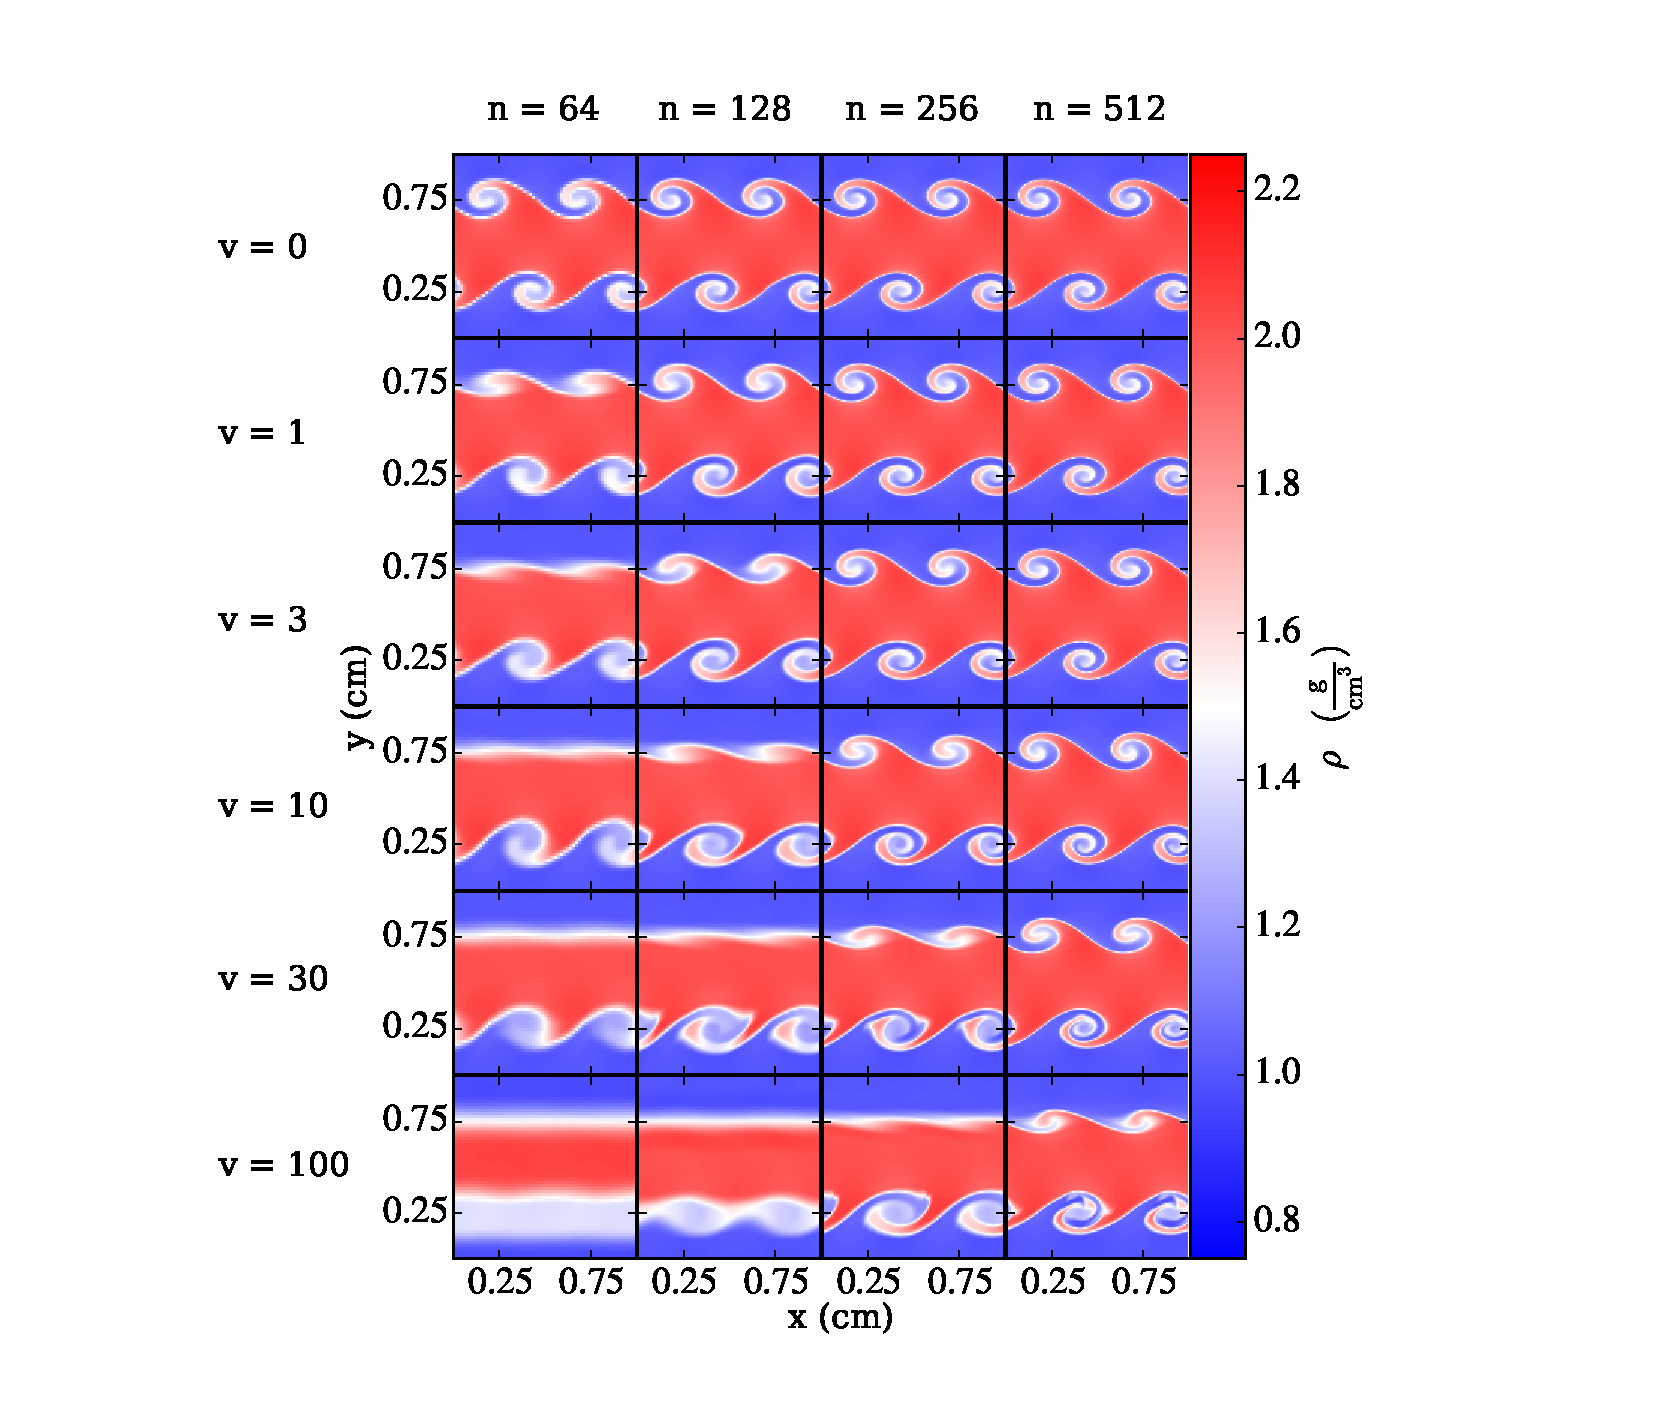
\includegraphics[trim=0.75in 0.45in 0.85in 0.5in, clip, scale = 0.75]{{{plots/kh_t2.0_p3_low_res_collage}}}
  \caption{2D Kelvin-Helmholtz instability test at $t = 2.0$ for the initial 
    conditions given by \autoref{eq:kh_p3_rho} through \autoref{eq:kh_p3_vy}. 
    The meaning of the rows and columns is the same as in \autoref{fig:kh_p2}.
    \label{fig:kh_p3}}
\end{figure*}

Here $w_0 = 0.1$ is the scale of the velocity perturbation, $\sigma =
0.05/\sqrt{2}$ controls the width of the Gaussian for IC A, and
$\Delta y = 0.05$ is the transition distance scale for the smooth ramp of IC
B. The pressure everywhere is set to $p = 2.5$, and we run this with a
gamma-law equation of state set to $\gamma = 5/3$. Plotfiles are
generated every 0.05 seconds, and the problem is run until $t = 2$.

We run the problem for $v_\text{bulk} = [0, 1, 3, 10, 30, 100]$, and
for each set of initial conditions run the problem at resolutions of
$64^2$, $128^2$, $256^2$, $512^2$. For context, in these units the 
sound speed is $c\approx 0.7$. In addition, for each initial
condition we run simulations at the higher resolutions of $1024^2$,
$2048^2$, and $4096^2$ for the stationary problem only. These serve 
as a reference solution to gauge the extent to which the bulk flow 
affects the development of the fluid instability, and to determine 
if the problem is numerically converged.

We find the same result as R10 for IC A, which is equivalent to the 
test proposed by S10: at low resolutions and high bulk velocity, the 
Kelvin-Helmholtz instability completely fails to develop. However, 
the problem does not converge even qualitatively at the highest 
resolutions we used. Our results are very similar to Figure 3 of 
R10 so we do not show them here. For IC B, our results can be seen 
for the normal resolutions and all velocities in \autoref{fig:kh_p2}.
At low resolutions and very large bulk velocities, the fluid 
does get significantly disrupted by numerical error. However, this 
effect quickly converges away with resolution and qualitatively 
at $512^2$ resolution the solution is nearly identical to the stationary 
$v=0$ problem. We agree with R10 that this problem does converge 
with resolution and is not subject to numerically-seeded secondary 
instabilities at the stopping time. This is evident even at low resolutions
by examining the first row of \autoref{fig:kh_p2}.

\begin{figure*}[ht]
  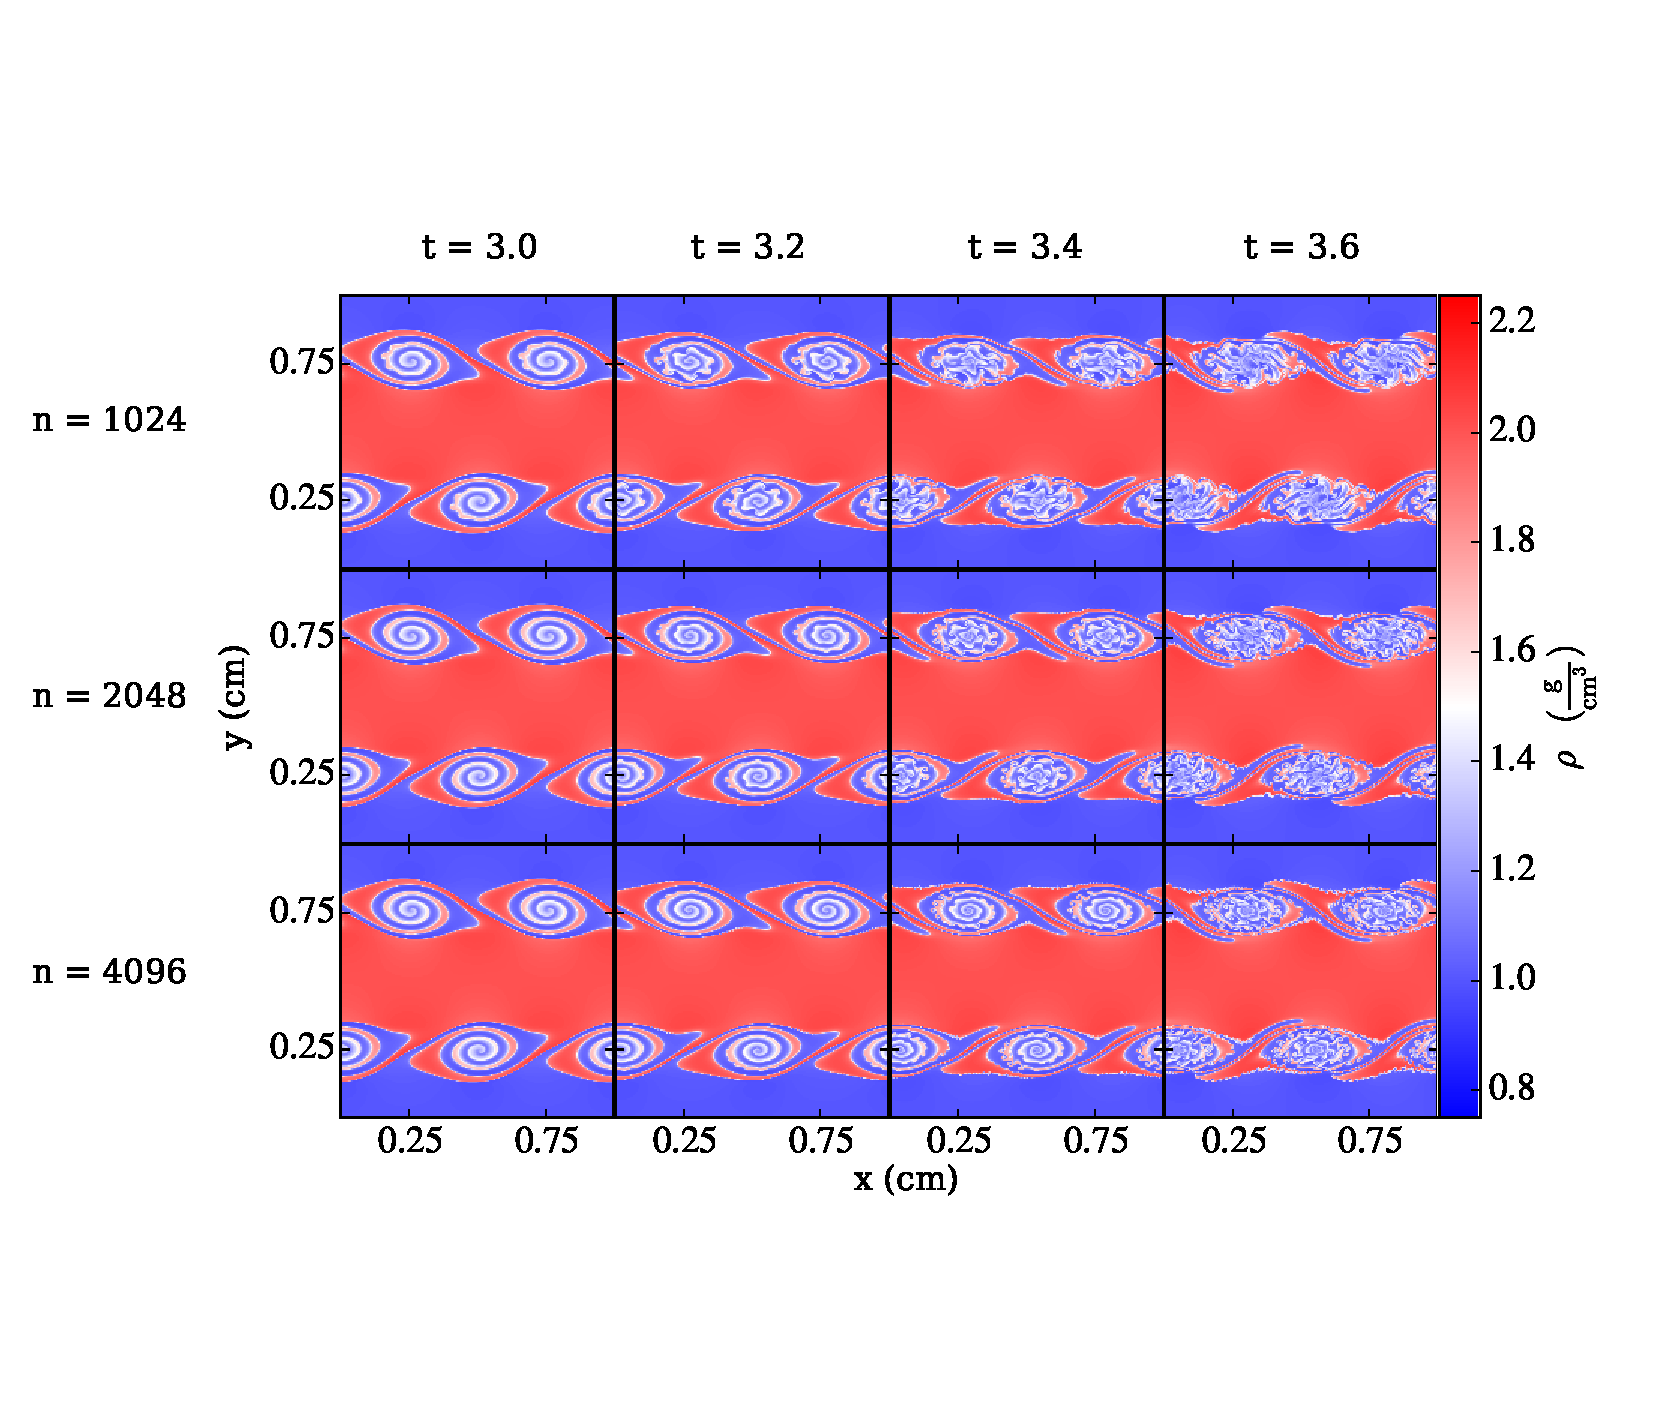
\includegraphics[trim = 0in 1.25in 0.25in 1.25in, clip, scale=0.65]{{{plots/kh_p3_high_res_collage}}}
  \caption{Time series of the Kelvin-Helmholtz problem proposed by McNally et al. (2012)
    as the simulation is just starting to go non-linear. The rows represent resolution, 
    where $n$ is the number of grid cells per spatial dimension, and the columns are 
    different snapshots in time.\label{fig:kh_p3_high_res}}
\end{figure*}

\citet{mcnally:2012} published another Kelvin-Helmholtz problem that 
is well-posed in the sense that it converges with resolution and 
is not subject to uncontrollable numerical instabilities. Though they 
were not explicitly interested in the question of Galilean invariance, 
we visit that issue here to see what can be learned. The initial 
conditions for this problem are:
\begin{align}
  \rho &= \begin{dcases} \rho_1 - \rho_m e^{(y-0.25)/\Delta y} & 0.25 > y \geq 0 \\ 
                         \rho_2 + \rho_m e^{(0.25-y)/\Delta y} & 0.5 > y \geq 0.25 \\
                         \rho_2 + \rho_m e^{(y-0.75)/\Delta y} & 0.75 > y \geq 0.5 \\
                         \rho_1 - \rho_m e^{(0.75-y)/\Delta y} & 1 > y \geq 0.75 \end{dcases} \label{eq:kh_p3_rho}\\
  v_x &= \begin{dcases} v_1 - v_m e^{(y-0.25)/\Delta y} & 0.25 > y \geq 0 \\
                        v_2 + v_m e^{(0.25-y)/\Delta y} & 0.5 > y \geq 0.25 \\
                        v_2 + v_m e^{(y-0.75)/\Delta y} & 0.75 > y \geq 0.5 \\
                        v_1 - v_m e^{(0.75-y)/\Delta y} & 1 > y \geq 0.75 \end{dcases} \label{eq:kh_p3_vx} \\
  v_y &= w_0\, \text{sin}\left(4\pi x\right). \label{eq:kh_p3_vy}
\end{align}
Here $\Delta y = 0.025$, $w_0 = 0.01$, $v_m = (v_1 - v_2) / 2$, $\rho_m = (\rho_1 - \rho_2) / 2$, 
and the other symbols have the same meaning as above (this means the flow direction
is reversed compared to the original paper, so as to achieve consistency with the 
other simulations presented here). We run this problem at all the same resolutions 
and bulk velocities as the previous two problems. The results for the normal resolutions 
at $t = 2.0$ are displayed in \autoref{fig:kh_p3}. We see a similar pattern as for 
the test proposed by R10: as we get to higher flow speeds we need to have higher 
spatial resolution to compensate for the increased numerical diffusion. However, 
the accuracy is much lower for the highest bulk velocities. This is probably because 
the initial conditions feature a transition that is twice as sharp (compare the $\Delta y$ 
parameters in each case). This means that there are smaller scale numerical 
perturbations on the grid, which can be amplified by numerical noise in the time 
evolution of the system.

\citet{hopkins:2015} performed this test as part of the testing of their code GIZMO. 
They showed the late-time evolution of this system, when non-linear effects have 
taken over and significantly disrupted the initial flow. However, at low resolution the 
tested grid algorithm had failed to disrupt both for $v = 0$ and $v = 10$. We too ran 
this problem until $t = 10$, and confirm that the Kelvin-Helmholtz instability damps out 
at low resolution but goes strongly non-linear and disrupts the flow at high resolution.
However, we strongly emphasize the point that this does not objectively 
demonstrate a defiency in fixed-grid codes for this problem. We can only determine 
the validity of a method when we have a trustworthy, converged solution to compare to, and 
this is lacking for this problem at late times. As observed by \citeauthor{mcnally:2012}, 
this is because the secondary instabilities form for this problem when the whorls of 
the Kelvin-Helmholtz tendrils stretch out and create gradients that approach the 
grid resolution. This is prime breeding ground for numerical noise. But because 
the nature of this noise will depend on the resolution, it will be very different for 
simulations at different resolutions. If these instabilities are seeded because of 
this resolution-dependent noise and are not seeded instead in a controlled manner 
such that they appear at the same time and location, then we simply cannot draw 
any conclusions that bear on the question of verification from this test at late times. 
\autoref{fig:kh_p3_high_res} provides a sense of this by examining the crucial 
time at which the transition from the linear to the non-linear regime is occurring. 
At all of these very high resolutions the secondary instabilities develop, but they 
occur at different times and have different spatial scales for each resolution.

We conclude that large bulk motions of fluid can have very significant effects 
on numerical calculations of shear mixing in fixed-grid codes, but that this effect 
diminishes with increasing resolution. As a result, we need only be confident that we are 
sufficiently resolving the major mixing regions on the white dwarf surfaces. 
If we find that this mixing occurs near the grid resolution scale, this will imply 
that we need to ramp up the resolution in these regions using AMR. If this becomes 
too expensive, we would need to be skeptical of any conclusions that could be drawn 
about the effect of the mixing on the nuclear burning.

\subsubsection{Moving Star}\label{sec:moving_star}

To see this effect in action for a stellar simulation, we repeated the test of  
\autoref{sec:HSE} with a bulk velocity on the grid. We chose a velocity of $2.56 \times 10^{8}\ \text{cm s}^{-1}$.
For context, this is comparable to the orbital velocities of the stars in \autoref{sec:kepler}.
This test was inspired by \citet{tasker:2008}, who considered a moving galaxy cluster 
and who obtained a long timescale evolution by using periodic boundary conditions, 
so that the cluster would cross the domain multiple times throughout the evolution.
We believe that periodic boundary conditions are unrealistic for our type of simulation,
so we prefer to do one continuous simulation where the star does not cross the boundaries.
Since our normal grid was not large enough to allow the motion to continue for very long, we expanded 
the domain size by a factor of four, and then included an extra refined level around the star to 
keep the effective resolution the same. We started the star off in the lower left corner of the domain, and 
pointed its velocity towards the upper right corner. This allowed us to evolve the star for the 
same length of time as for the original test. We note that getting the gravity boundary conditions right 
required us to move the origin of the problem at the bulk velocity, so that the multipole moments 
were computed with respect to the stellar center.

\begin{figure}
  \centering
  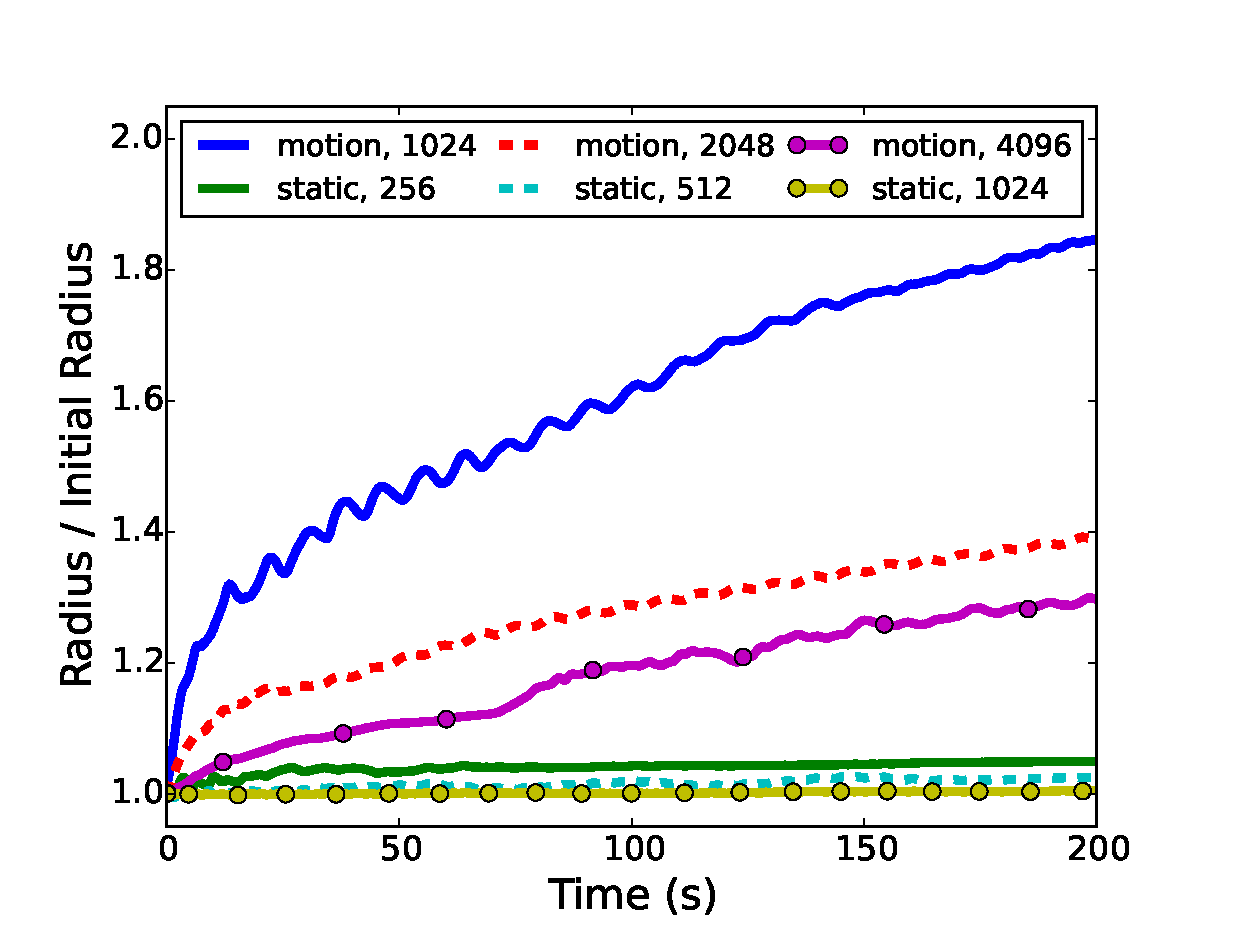
\includegraphics[scale=0.45]{plots/single_star_compare_1e3_radius}
  \caption{A variation on \autoref{fig:single_star_static_radius} where
    we now compare the ``static'' case to ``motion'' simulations where the 
    star moves across the grid at a fixed linear speed. The lines represent 
    the effective number of zones per dimension inside the stellar material;
    due to the expanded size of the grid in the ``motion'' case, the 
    physical resolution is the same in each column in the legend.
    \label{fig:single_star_compare_radius}}
\end{figure}

In \autoref{fig:single_star_compare_radius}, we take the results of 
\autoref{sec:HSE} (the ``static'' case), and plot on top of it the results of this 
new simulation (the ``motion'' case). We see immediately that this bulk velocity
causes the star to be much worse at maintaining hydrostatic equilibrium. Not only 
is the absolute size of the star significantly larger (nearly a factor of two 
at the lowest feasible resolution we consider), but also there is a clear upward 
trend in the size that has not terminated at any resolution by the end of the simulation.
This again emphasizes the results mentioned earlier, that we must be careful not 
to trust any simulation with significant mass transfer if we are not confident that the 
mass transfer is seeded in a controllable manner and free from numerical noise.

\subsection{Keplerian Orbit}\label{sec:kepler}

We now consider the phase of the binary system where the stars are orbiting each other 
at distances great enough that the initial orbits should be approximately Keplerian. 
There are a number of effects worth looking into here. For simplicity, we choose two 
cases to demonstrate the simulation behavior: an equal mass case of two $0.9\msolar$ 
white dwarfs, and an unequal mass case of $0.9\msolar$ and $0.6\msolar$ white dwarfs.
In each case, the initial orbital period is 100 seconds.

For some of the algorithms described earlier in this work, a single orbit of these 
systems is enough to examine their effects. In \autoref{sec:gravity_boundary_conditions},
we discussed the replacement of a monopole boundary condition solver for the gravitational 
potential with a more general multipole solver for the boundaries. To test the relevance 
of this effect, we considered a single orbit of the unequal mass system and measured 
the distance between the two white dwarfs at the beginning of the simulation and after 
the full orbital period. This distance should not change significantly over that timescale.
We performed this test for maximum multipole moments ranging from 0 (the monopole term) to 16.
The results are shown in \autoref{fig:gravity_bcs}. Terms in the boundary potential 
that vary faster than $r^{-5}$ are effectively negligible in determining the outcome of the orbit, 
justifying our typical choice of maintaining terms up to $r^{-7}$.

\begin{figure}
  \centering
  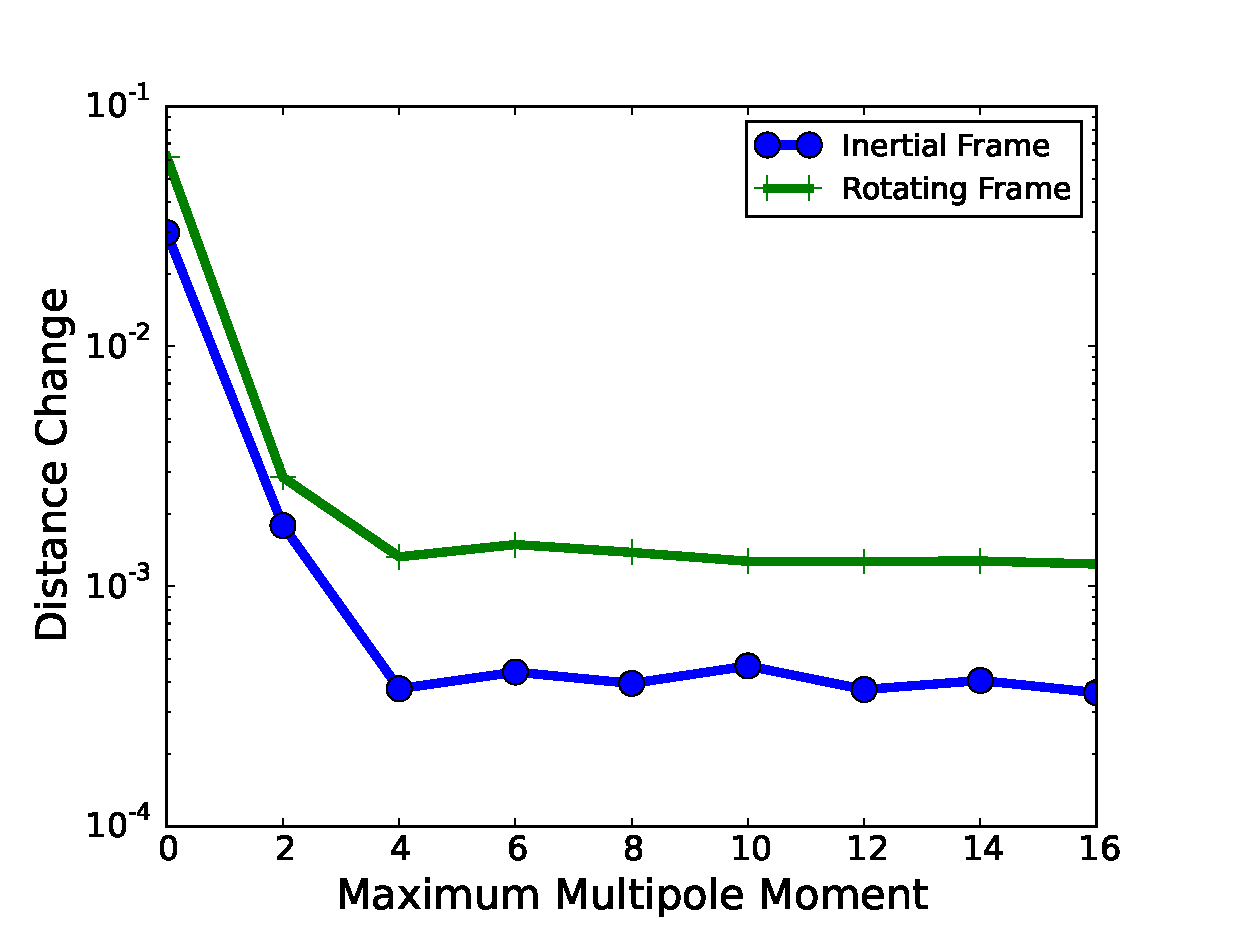
\includegraphics[scale=0.45]{plots/gravity_bcs}
  \caption{Absolute magnitude of the relative change in the distance of two unequal mass white dwarfs after one orbital period. 
           The stars were evolved in an inertial reference frame. The horizontal axis is the number of terms or multipole moments 
           captured in the series expansion for the potential at the domain boundary.\label{fig:gravity_bcs}}
\end{figure}

Another that we consider is the energy conservation of the system. Recalling \autoref{sec:gravity_hydro_coupling}, 
there are several different methods of applying the gravitational source term to the hydrodynamics equations. In \castro\ we presently 
have four options, controlled by the parameter {\tt castro.grav\_source\_type}, which we will shortern to {\tt gs} for the present 
discussion. ${\tt gs} = 1$ is the standard cell-centered source term for gravity. ${\tt gs} = 2$ is a slight variation on this scheme 
that determines the value of the energy source term after the momentum source term has been applied; the former approach uses 
the uncorrected momenta in calculating $\rho \mathbf{u} g$, which we have found to be more accurate. ${\tt gs} = 3$ is entirely 
different: after calculating the new momenta, we reset the total energy to be equal to the internal energy plus the 
kinetic energy. This has the virtue of ensuring that there is no conflict due to discretization between the momentum and 
energy equations, and also correctly ensuring that the gravitational force does not directly change the internal energy -- 
and thus the temperature -- of the fluid. However, it explicitly sacrifices total energy conservation. ${\tt gs} = 4$ is 
the new conservative method of evaluating the energy source terms at cell faces. The results for the change in energy 
after a single orbit are seen in the first column of \autoref{table:sources}. The first two versions give reasonable and 
similar levels of energy conservation. The third has total energy changes on the order of 100\%, but this itself 
does not have a severe effect on the dynamics because in this scheme the total energy variable is effectively a placeholder 
value of the kinetic energy plus internal energy, rather than being evolved directly. The last scheme is nearly two orders 
of magnitude better in energy conservation, justifying the effort in varying the scheme.

In \autoref{table:sources} we show also the effects on energy conservation of using the inertial reference frame. 
We use ${\tt rs}$ for the \castro\ parameter {\tt castro.rot\_source\_type}, and we have the same four options for updating
the energy source term as for gravity. The ${\tt rs} = 0$ column means that rotation is turned off and we are 
in the inertial frame. We see that the choice of rotational coupling is much less important than the choice of gravity coupling. 
Interestingly, the ``conservative'' ${\tt rs} = 4$ is slightly worse in energy conservation than the non-conservative, 
cell-centered ${\tt rs} = 2$ algorithm. This may be because the rotational force grows with distance, and so losses at the 
domain boundaries may be enhanced by explicitly evaluating the flux at cell edges.

\capstartfalse
\input{plots/sources.table}
\capstarttrue

We are most interested in the stability of these systems over long timescales. To this end, we consider the same systems as above, 
but evolve them for 25 orbital periods. In \autoref{fig:circular_orbit_comparison} we illustrate the evolution of these systems 
by plotting the center of mass locations of the white dwarfs on the orbital ($xy$) plane. For the equal mass case in the inertial 
reference frame, the curves essentially fall on top of each other, indicating that the stars are indeed orbiting at the initial 
distance without substantial deviation. In the unequal mass case, the stars now orbit at different distances but do not much 
deviate from their initial distance. We do observe a secular decline in the center of mass of these stars, indicating that 
eventually the stellar orbits will degrade due to numerical error even without intervention. The co-rotating frame is different.
For clarity of visualization, we rotate these results back into the inertial frame before displaying their orbits.
The stellar orbit in the equal mass case does not show the same secular decline, and the system appears to be stable. However, 
the cost is that the oscillations about this equilibrium are slightly larger than in the inertial frame. The unequal mass case displays 
this effect starkly: while the average distance is not declining, there are huge oscillations about this average. In addition, 
the stars move substantially within the rotating frame itself, yielding the chaotic-looking orbits in the figure. The oscillations 
grow with time and will eventually cause the stars to merge; however, the stars would eventually merge even in the inertial frame 
case, and at a faster rate than the equal mass case. This suggests that this mass ratio is too large to ignore tidal effects, and 
that the tidal effects play out much differently in the rotating frame.

\begin{figure*}
  \centering
  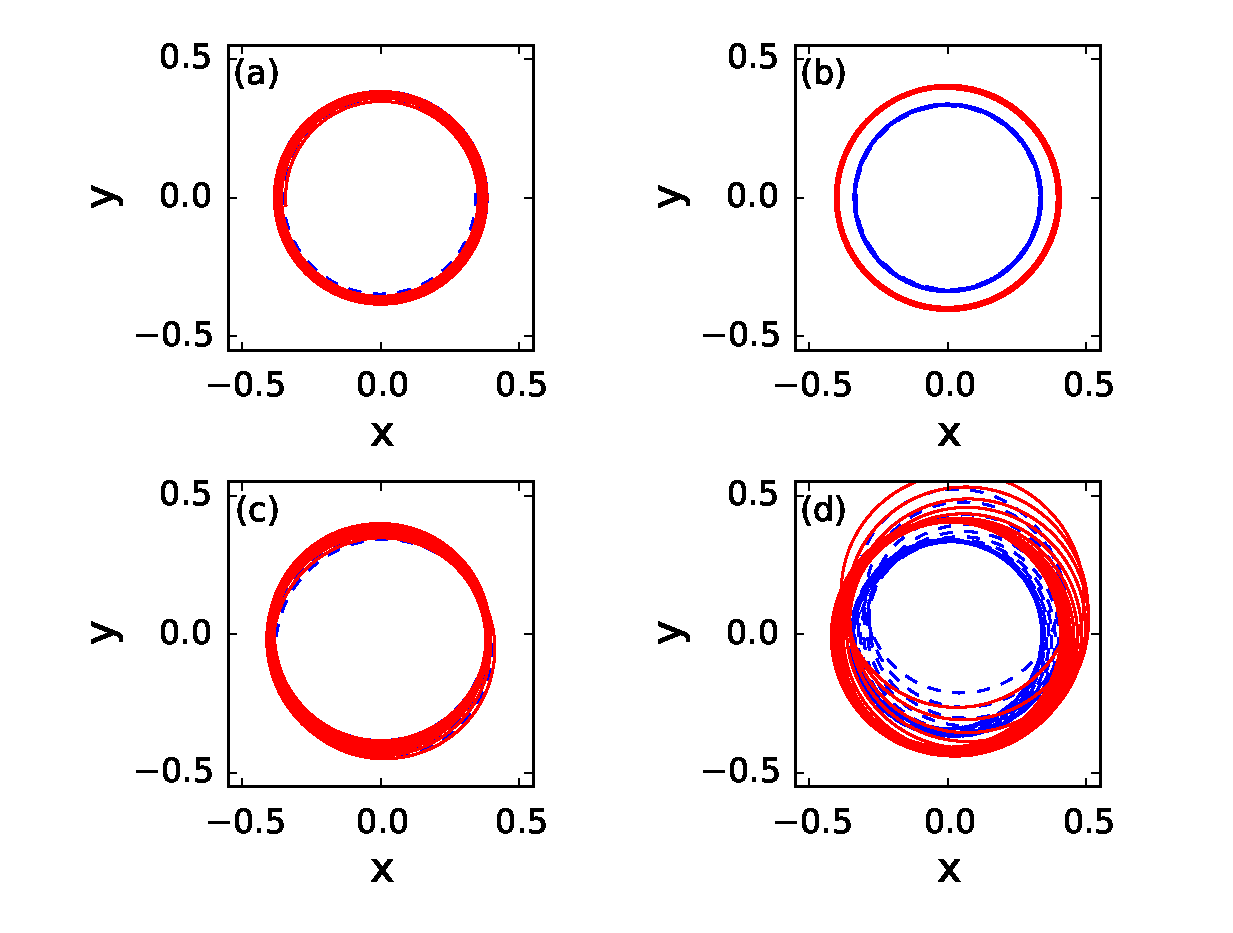
\includegraphics[scale=0.7]{plots/circular_orbit_comparison}
  \caption{Positions of the white dwarfs in the orbital plane for four cases evolved over 25 orbital periods. 
           The $x$ and $y$ axes are normalized to the size of the domain, so that $x = -0.5$ is the left edge 
           and $x = 0.5$ is the right edge. The dashed blue curve is the position of the primary white dwarf, 
           and the solid red curve is the position of the secondary. In plot (a) we have the equal mass system 
           evolved in the inertial reference frame, and in plot (c) we have the same system evolved in a rotating frame, 
           where the positions have been transformed back to the inertial frame for comparison. 
           Plots (b) and (d) are analogous but for the unequal mass system.\label{fig:circular_orbit_comparison}}
\end{figure*}

Turning to the conservation properties of the system, we examine as fairly typical cases the equal mass system 
in the inertial frame for energy conservation (\autoref{fig:energy_conservation_equal}), and the unequal mass 
system in the rotating frame for angular momentum conservation (\autoref{fig:angular_momentum_conservation_unequal}). 
Angular momentum is conserved to within a few percent over the 25 orbits, while energy conservation is about 
an order of magnitude better. We note that while this is already a fairly good level of energy conservation, it is not 
nearly as good as the results of \citet{marcello:2012}. This is because we reset the internal energy to a level 
corresponding to our temperature floor when it goes negative, while \citeauthor{marcello:2012} do not reset and 
instead ignore the internal energy if it is negative. The resets impose an artificial floor on our ability to 
conserve energy, but they only happen in low-density regions and do not much affect the large-scale dynamics. 
Meanwhile, angular momentum conservation is not quite as good. This is linked to the decline (or increase) in 
the size of the orbit. This implies that we ought to be careful in concluding that at these moderate resolutions 
we can safely evolve systems for many dozens of orbits; this needs to be verified to ensure that an observed 
inspiral and merger is physically (not numerically) motivated.

\begin{figure}
  \centering
  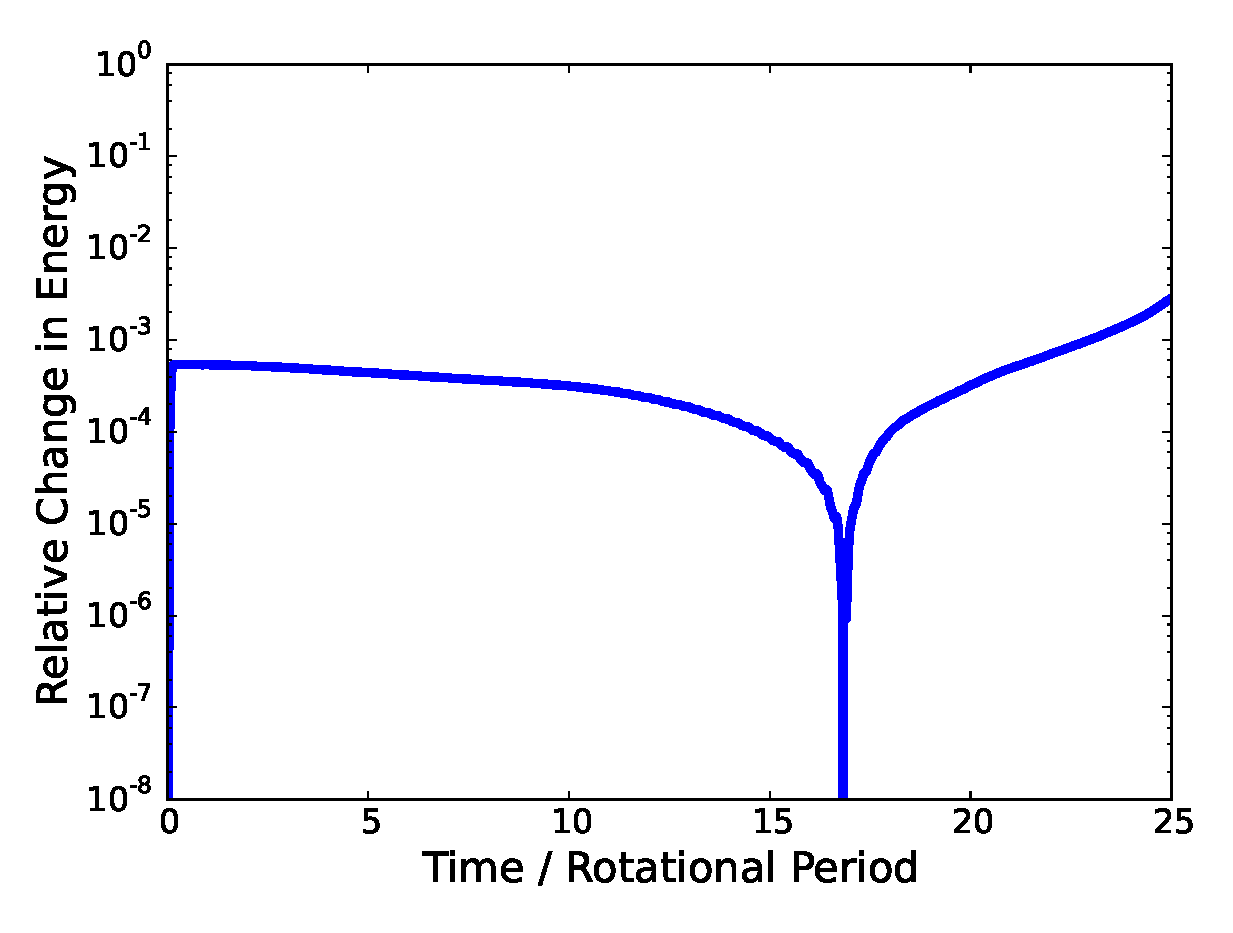
\includegraphics[scale=0.45]{plots/equal_energy_rot0.eps}
  \caption{Absolute magnitude of the relative change in energy of two equal mass white dwarfs through 25 orbital periods,
           evolved in an inertial reference frame. The decline and recovery is a change in sign of the energy difference.
           \label{fig:energy_conservation_equal}}
\end{figure}

\begin{figure}
  \centering
  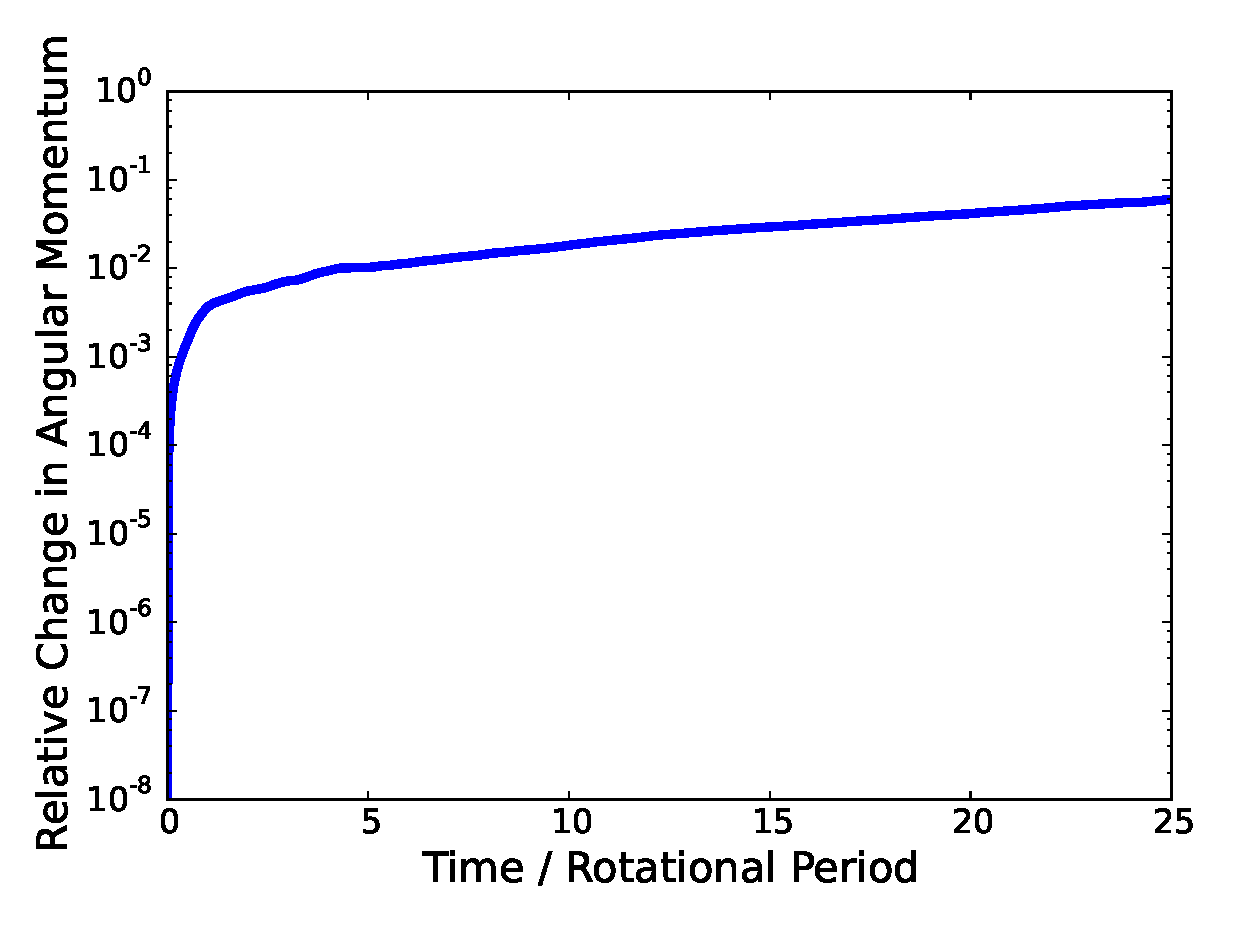
\includegraphics[scale=0.45]{plots/unequal_angular_momentum_rot1.eps}
  \caption{Absolute magnitude of the relative change in angular momentum of two equal mass white dwarfs after 25 orbital periods, 
           evolved in a co-rotating reference frame. We consider only the component of the angular moment along the rotational 
           axis. The decline and recovery is a change in sign of the angular momentum difference.
           \label{fig:angular_momentum_conservation_unequal}}
\end{figure}

As a simple verification test to ensure our gravitational wave calculations are correct, we plot the 
gravitational wave strain along the rotation axis for the first two periods of the unequal mass system. 
At this early time the orbit is circular and so to a good approximation we expect that the gravitational 
wave signal should be that of two point masses, whose positions are:
\begin{align}
  \mathbf{r}_P(t) &= -a_P\, \text{cos}(\omega t) \hat{x} - a_P\, \text{sin}(\omega t) \hat{y} \\
  \mathbf{r}_S(t) &= a_S\, \text{cos}(\omega t) \hat{x} + a_S\, \text{sin}(\omega t) \hat{y}.
\end{align}
Then the mass distribution is $\rho(\mathbf{r}) = M_P\, \delta^3(\mathbf{r} - \mathbf{r}_P) + M_S\, \delta^3(\mathbf{r} - \mathbf{r}_S)$.
From this it is straightforward to calculate the quadruopole tensor, take its second time derivative, and then apply the 
projection operator to get the gravitational wave polarizations along the rotation axis:
\begin{align}
  h_+ &= -4\frac{G\mu}{c^4 r}\left[G M_{\text{tot}} \omega \right]^{2/3}\, \text{cos}(2\omega t) \\
  h_\times &= -4\frac{G\mu}{c^4 r}\left[G M_{\text{tot}} \omega \right]^{2/3}\, \text{sin}(2\omega t).
\end{align}
$\mu$ is the reduced mass, while $M_{\text{tot}}$ is the total mass. From this we see that the 
gravitational wave frequency is twice the orbital frequency, and that the two polarizations 
are out of phase by $90^\circ$ in time. We compare this analytical expectation to the 
numerical results in \autoref{fig:gw_strain}. We find very good agreement in this case, and this 
level of agreement holds in the rotating frame as well.

\begin{figure}
  \centering
  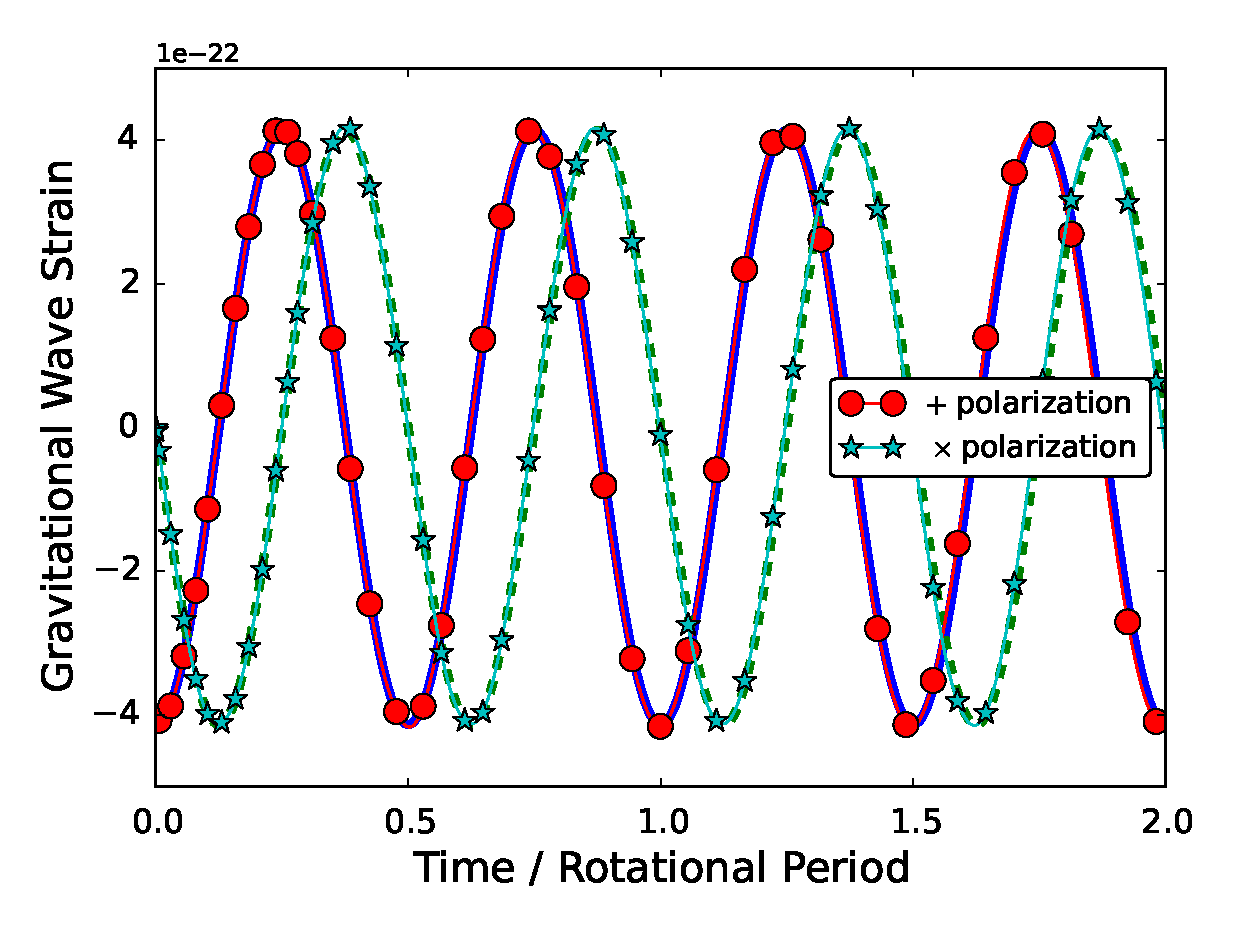
\includegraphics[scale=0.45]{plots/unequal_gw_rot0.eps}
  \caption{Gravitational wave strain polarizations for the first two orbital periods of the 
           unequal mass system. The curves with markers are the numerical data, while the 
           curves without markers are the analytical results for two point masses.\label{fig:gw_strain}}
\end{figure}

Finally we consider whether the dynamical behavior of the system converges with resolution. 
In \autoref{fig:unequal_spatial_convergence} we plot the first 10 seconds of the orbit for 
the unequal mass system, at three different resolutions in the inertial frame: our default 
resolution of $256^3$ zones, as well as a single level of refinement with a jump by a factor of 
two (effective resolution $512^3$) or a jump by a factor of four (effective resolution $1024^3$). 
It is clear that at the latter resolution (corresponding to physical resolution of 100 km), 
we have achieved convergent behavior. In the rotating frame (not shown here), the results are 
not quite the same but for these resolutions the results do tend toward convergence.

\begin{figure}
  \centering
  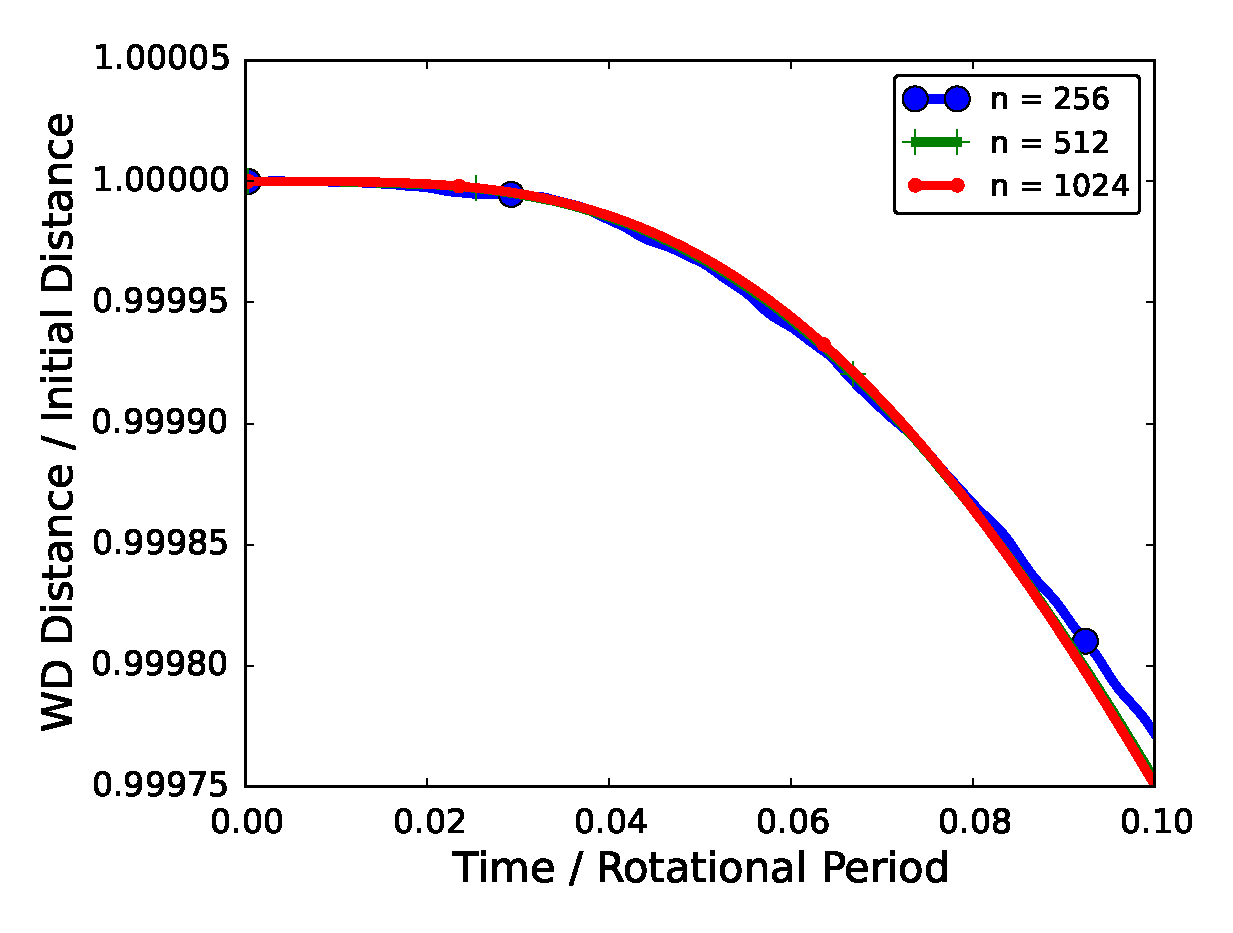
\includegraphics[scale=0.45]{plots/spatial_convergence_rot0.eps}
  \caption{Distance between the two white dwarfs in the unequal mass system, for the first 
           10 seconds of their orbit. The distance is scaled by the initial orbital distance. 
           We plot at three different resolutions, corresponding to the number of 
           effective zones per dimension in the refined regions. Note that the $n = 1024$ curve
           falls nearly exactly on top of the $n = 512$ curve.\label{fig:unequal_spatial_convergence}}
\end{figure}



%==========================================================================
% Performance
%==========================================================================
\section{Parallel Strategy and Performance}\label{sec:Performance}

\castro\ is designed to be deployed on high-performance computing systems using 
many thousands of processors simultaneously. It is worth briefly examining 
our strategy for parallelizing the problem over many computational nodes 
and our performance in situations similar to production science simulations. 
This is especially true because some aspects of our approach to parallelism 
have changed since the first \castro\ paper, and we have obtained improved 
performance in certain settings.

The \boxlib\ framework that \castro\ is based on splits each AMR level into a number 
of boxes that collectively span the level. These boxes are distributed to processors 
through MPI parallelism; each MPI task in general holds multiple boxes and 
an update includes a loop over all the boxes an MPI task owns. The distribution 
obeys a load-balancing algorithm that attempts to equalize the amount of work 
done by each processor. \boxlib\ contains a number of strategies for distributing 
work in this way, and by default uses a space-filling curve approach with a 
Morton ordering. By experiment we have found that the most efficient load-balancing 
strategy for our problem is actually a simple knapsack algorithm. In this approach, 
the amount of work owned by a processor is proportional to the number of grid cells 
associated with that processor, and the algorithm attempts to ensure that all 
processors have a similar number of total grid cells. We demand an efficiency of 0.9,
meaning that the average workload per processor should be no smaller than 90\% of the 
maximum workload found on any processor. However, we find that in practice the 
performance is largely insensitive to this choice.

The size and shape of grid boxes is an important consideration for efficiency. 
Boxes that are very small suffer from a host of problems, including the larger 
amount of communication required between hydrodynamics solves. Additionally, 
the multigrid solver will be less efficient if the boxes are small because there 
will be fewer available levels for coarsening and performing V-cycles. Conversely, 
boxes that are too large mean that there isn't enough work to go around when we 
have a large number of processors. Good performance is the result of a careful 
balance between these two effects. On the lower end, we require that all boxes 
be a multiple of 16 zones in each dimension; multigrid efficiency sharply decreases 
if this factor is any lower. On the upper end, we select the maximum grid size 
based on the number of processors we use and the total number of cells in the 
simulation. This size will therefore in general vary on different AMR levels. 
Generally we select a value in between 32 and 64 zones per dimension.

We use OpenMP to accelerate the work associated with the boxes owned by each 
MPI task. Originally \castro\ used OpenMP to accelerate individual loops in the 
hydrodynamics routines, such as the piecewise-parabolic edge state reconstruction 
and the conservative flux update. However, there is a significant amount of 
overhead associated with generating a new OpenMP region at each of the many 
different loops in a hydrodynamics algorithm. This makes such a strategy 
sub-optimal for use on many-core processors and GPUs. We have recently switched 
to a tiling approach, where an OpenMP region is generated at the start of 
the hydrodynamics routine and the individual threads separately work on 
different partitions of each box. This results in much less overhead for 
the threading. In general we obtain more efficient simulations than 
could be obtained using MPI only, because there are fewer boxes and thus 
less communication for a given number of processor cores. We are currently 
developing an approach to evaluating the equation of state and nuclear reactions 
(and possibly the entire hydrodynamics algorithm) on GPUs, which will allow us
to take advantage of the significant computational resources embedded in GPUs on 
certain systems.

\begin{figure}
  \centering
  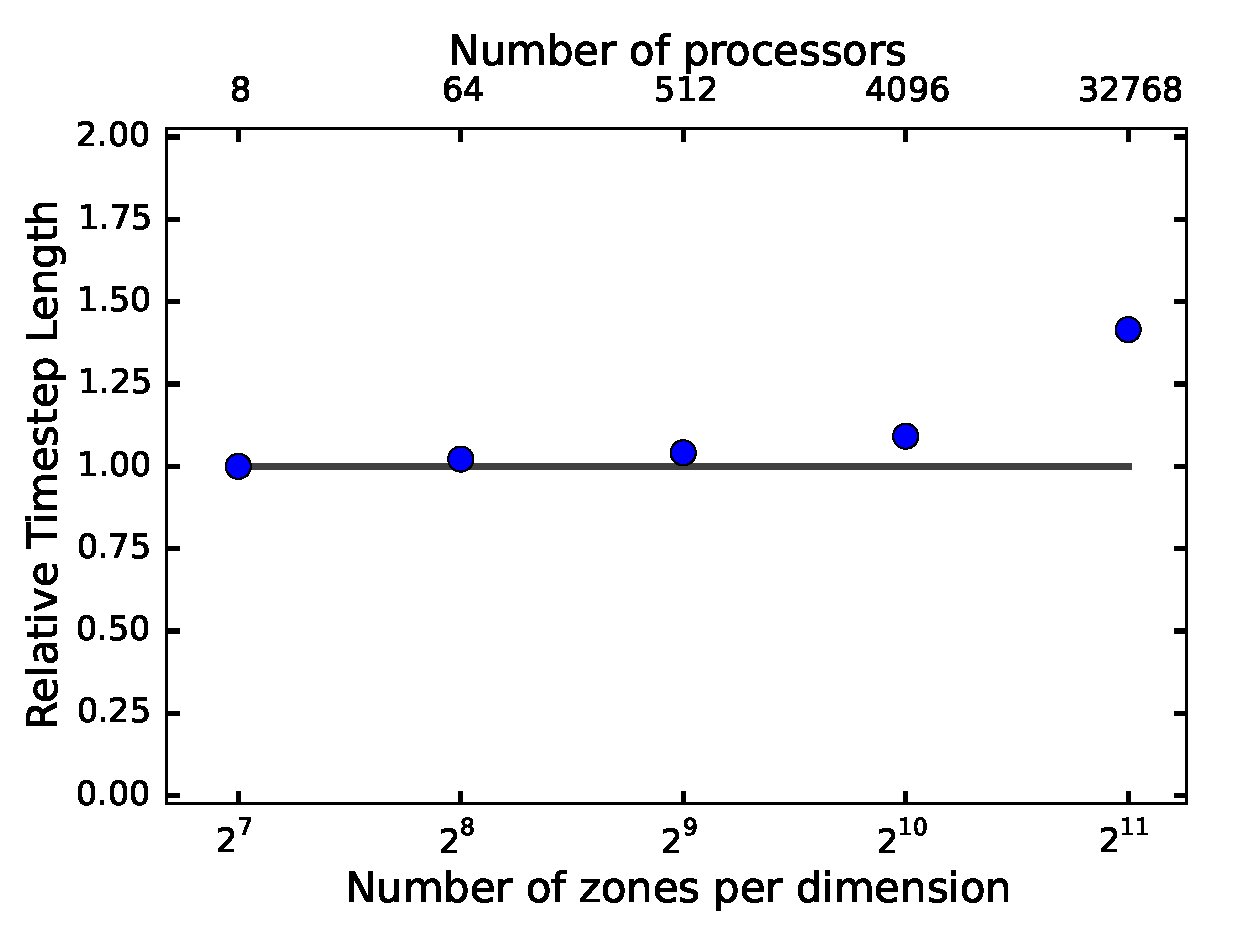
\includegraphics[scale=0.4]{plots/weak_scaling}
  \caption{\castro\ weak scaling test, performed on the Blue Waters machine at 
    NCSA. Each processor had a fixed amount of work, and we increased the 
    number of simulation zones in concert with the number of processors. The 
    solid curve represents perfect weak scaling, while the blue circles show 
    \castro's performance at each processor count. The vertical axis measures 
    the median time per timestep, normalized to this value for the smallest 
    processor count.\label{fig:weak_scaling}}
\end{figure}

To examine the parallel performance of \castro, we performed both strong scaling 
and weak scaling tests on the Blue Waters machine at the National Center for 
Supercomputing Applications. For the weak scaling test, whose results are 
shown in \autoref{fig:weak_scaling}, we ran a uniform grid binary white 
dwarf simulation for resolutions of $128^3$ zones through $2048^3$ zones. The 
number of processors was scaled with the number of zones so that each processor 
had the same amount of work; the smallest test used 8 processors and the largest 
used 32,768 (note that the number of processor cores on a Blue Waters node is twice 
the number of floating point units on that node). The test was run for 10 timesteps,
with each timestep including two Poisson solves and a hydrodynamics update (though 
for a uniform grid calculation we generally do not need to perform any multigrid 
iterations for the first Poisson solve in a timestep, since the density distribution 
has not changed since the end of the last timestep). We disabled plotfile and 
checkpoint writing, as well as calculation of diagnostic information (the latter 
can contribute to a significant fraction of the run time at large processor 
counts if computed every timestep). We computed the median wall time required per 
time step for each simulation, and then normalized this to the median time per 
timestep for the smallest simulation. We find excellent weak scaling through 
4,096 processors. At the largest run, the simulation time required is 
more than 1.5 times the amount required for the smallest simulation. 
This is due entirely to the increased cost of the multigrid Poisson solve 
in each timestep and this cannot be mitigated except by improving 
communication or computation efficiency in the multigrid solver. We observe 
that this weak scaling behavior with Poisson gravity is a significant 
improvement over the results presented in the first \castro\ paper.

\begin{figure}
  \centering
  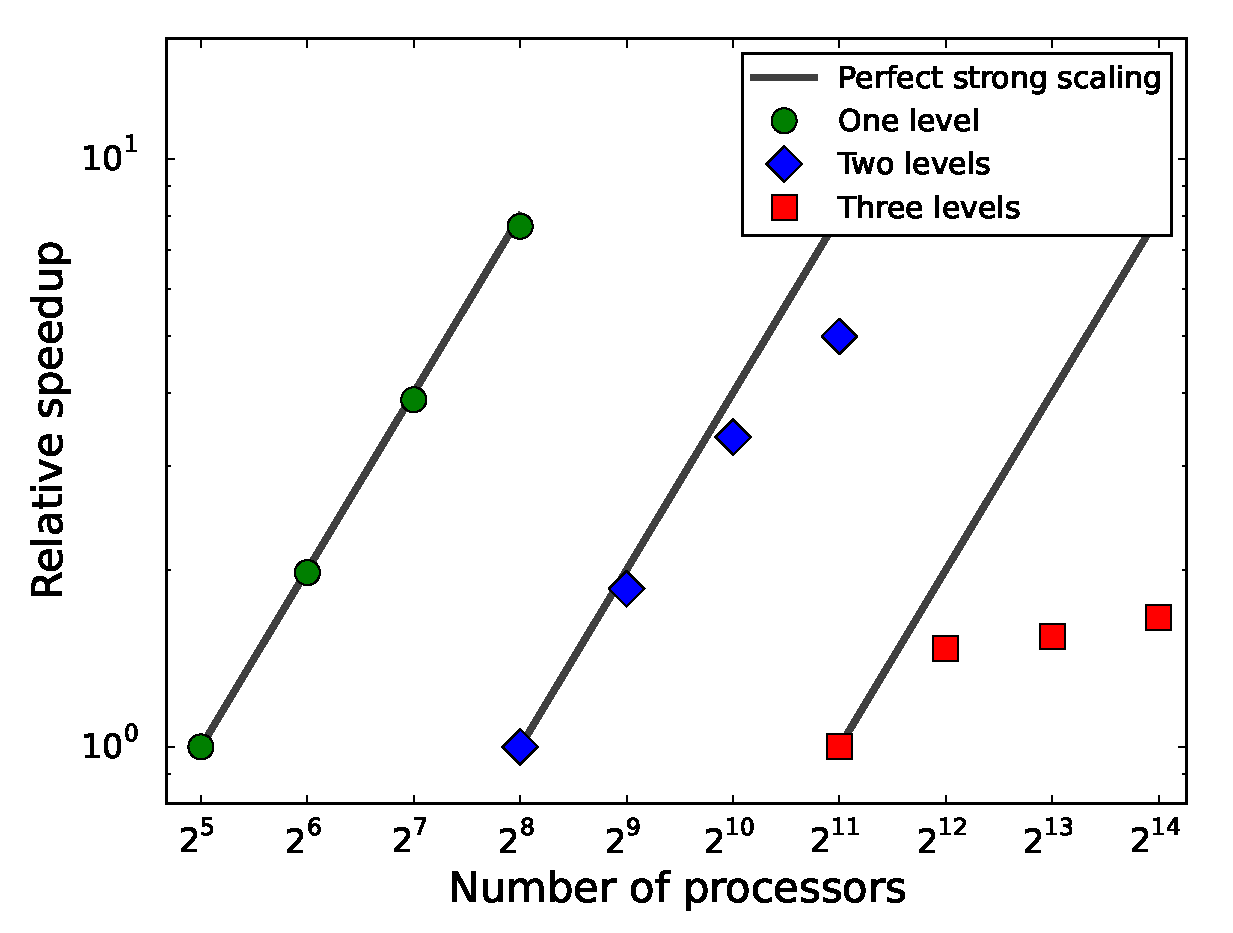
\includegraphics[scale=0.4]{plots/strong_scaling}
  \caption{\castro\ strong scaling test performed on the Blue Waters machine at
    NCSA. The vertical axis measures the median time per timestep, and the 
    horizontal axis measures the number of processors in the simulation. Data 
    points are normalized to the time per timestep for the smallest number 
    of processors. The blue circles show the data for a simulation with two AMR
    levels (one coarse and one fine), while the red circles show the data 
    for a test with three AMR levels (one coarse and two fine). The fine levels 
    increase the resolution only in the regions around the stars. For each case 
    we draw a solid curve representing perfect strong scaling.\label{fig:strong_scaling}}
\end{figure}

The strong scaling test we perform uses a grid setup similar to what we 
use for well-resolved binary simulations. With a single refined level, 
we have approximately $5 \times 10^7$ zones spread over $\sim 1000$ grids.
On a second refined level, there are $2 \times 10^9$ zones spread over 
$\sim 16000$ grids. We run a scaling test for both cases, with the 
highest processor count in each case chosen so that the number of 
MPI tasks is similar to the number of grids. There are no relative gains 
to be achieved from further parallelism. The results are found in 
\autoref{fig:strong_scaling}. We find excellent scaling for low numbers 
of processors, though the long wall time per timestep required for the 
smallest processor counts makes such a simulation infeasible in practice.
The best tradeoff between reasonable wall time and parallel efficiency 
seems to be when there are approximately 2--4 grids per processor. The 
scaling behavior worsens at the highest processor counts, but this is 
an expected consequence of processors becoming work-starved. In general 
we find very good strong scaling behavior in the regime we are presently 
interested in, simulating the early phases of a simulation at moderate 
resolution. The strong scaling behavior is acceptable, though not perfect, 
at very large processor counts when self-gravity is considered.

%==========================================================================
% Conclusions
%==========================================================================
\section{Conclusions and Discussion}\label{sec:Conclusions and Discussion}

In this paper we have described the major components of a framework for 
simulating mergers of white dwarfs. While there is much evidence for the 
hypothesis that mergers (or collisions) of white dwarfs are significant 
contributors to the rate of Type Ia supernovae and related astronomical 
transients, the theoretical view on these systems is far from complete. 
Studying these systems over the long timescales relevant to dynamical 
mass transfer requires careful attention to the numerical methods used, 
to ensure that numerical instabilities or other errors do not unduly 
influence the system. Here we have described a number of common problems
that may creep up, including violation of the conservation of energy, 
a lack of hydrostatic equilibrium (at low resolution) of the stars 
even when not acted on by external gravitational forces, and large 
velocities that can be generated near the edges of stars due to the 
numerically sharp gradients. Some of the issues are simply unresolvable
at the resolutions achievable on modern supercomputing systems; 
for example, it is very difficult to adequately resolve the stellar 
surface of a white dwarf on a three-dimensional grid, and there is 
justifiable room for suspicion regarding what happens there. But others
are avoidable with care: energy non-conservation can be substantially 
mollified by using a form of the gravitational work that is explicitly 
conservative, and we have observed that this can be done for rotation 
source terms too.

We presented a set of numerical tests that show where we can 
and cannot trust these techniques. We spent much time considering 
the role of bulk motions on the grid and we conclude that there 
are real issues with substantial bulk velocities on static grids, 
that can diminish the quality of the resulting solutions to the 
fluid equations. However, these effects diminish with increasing 
resolution. We therefore make no explicit claims about the usefulness 
of Langrangian versus Eulerian methods and instead simply observe 
that whenever a simulation is performed, it is important to have 
a measure of numerical accuracy and a sense of whether we are 
witnessing properties that converge with increasing resolution.
These problems do suggest that, where possible, we should seek to 
minimize bulk motions on static grids. A comparison of orbit 
simulations in both rotating and inertial reference frames 
demonstrates that in practice this is not so simple, and that 
a rotating reference frame has its own numerical issues for 
the type of simulation we desire to perform here. Based on 
the tests performed here, in some cases the stars may be 
\textit{more} stable in an inertial frame despite 
constantly being in motion on the grid. It 
is not easy to predict the correct behavior of such systems, 
though one recourse for assessing confidence in a model from a 
verification standpoint is to see whether the observed 
behavior converges with resolution. However, it is not clear 
whether at practical resolutions the results in the 
rotating and inertial frames will converge to each other.

Future work on this project will focus on how to build 
reliable equilibrium initial models of the stars and 
an examination of how the mass transfer episode depends on 
these initial conditions, and then to enable the nuclear 
reaction network and determine whether self-consistent 
thermonuclear detonations are ignited and result in 
events that appear similar to Type Ia supernovae. Other 
areas ripe for future study include: the effect of radiation 
on the merger process; the extent to which the result 
depends on the initial composition of the stars (for example, 
by including surface layers of helium and/or by using 
white dwarf models generated by modern stellar evolution 
codes); the gravitational wave signals generated by 
white dwarf mergers; and, collisions of white dwarfs. All of 
these are possible under the framework we have established.

\acknowledgments

The authors thank Noel Scudder and Platon Karpov for their help with 
this project, especially related to visualization of the results. 
We also thank Adam Jacobs for his advice on and assistance with 
running on supercomputing resources. Special thanks are given 
to the organizers of the 2015 Caltech Gravitational Wave 
Astrophysics School, and their supporters: the NSF 
under CAREER award PHY-1151197, the Sherman Fairchild 
Foundation, the LIGO Laboratory at Caltech, and Caltech.

This research has made use of the AstroBetter blog and wiki. 
This research has made use of NASA's Astrophysics Data System 
Bibliographic Services.

This research was supported by NSF award AST-1211563. An
award of computer time was provided by the Innovative and Novel
Computational Impact on Theory and Experiment (INCITE) program.  This
research used resources of the Oak Ridge Leadership Computing Facility
located in the Oak Ridge National Laboratory, which is supported by
the Office of Science of the Department of Energy under Contract
DE-AC05-00OR22725. Projects AST006 and AST106 supported use of the ORNL/Titan resource. 
This research is part of the Blue Waters sustained-petascale computing project, 
which is supported by the National Science Foundation (awards OCI-0725070 
and ACI-1238993) and the state of Illinois. Blue Waters is a joint 
effort of the University of Illinois at Urbana-Champaign and its 
National Center for Supercomputing Applications.
This research used resources of the National Energy Research Scientific Computing
Center, which is supported by the Office of Science of the
U.S. Department of Energy under Contract No. DE-AC02-05CH11231.  
This work used the Extreme Science and Engineering Discovery Environment (XSEDE), 
which is supported by National Science Foundation grant number ACI-1053575. 
Project AST100037 supported use of the resources NICS/Kraken and NICS/Darter.

\clearpage

\appendix

\section{CASTRO hydrodynamics changes}

The basic PPM algorithm in \castro\ has undergone a number of changes
since the original code paper \citep{castro}.  A discussion of the
pure hydrodynamics changes along with verification of \castro\ when
using the stellar equation of state was given in
\citet{zingalekatz:2015}.  Here we discuss the changes that affect
multispecies flow and source terms.

\subsection{Reference States}

For all the runs, the PPM reconstruction is done using the original limiters for
the parabolic profiles \citep{ppm}; see \autoref{sec:Hydrodynamics} for a brief 
discussion about the limiters.  The prediction of the interface
states appears as:
\begin{equation}
\label{eq:ppmstatel}
q_{i+1/2,L}^{n+1/2} = \tilde{q}_L -
   \sum_{\nu;\lambda_i^{(\nu)}\ge 0} l_i^{(\nu)} \cdot \left [
        \tilde{q}_L  - \mathcal{I}^{(\nu)}_+(q_i)
       \right ] r_i^{(\nu)}
\end{equation}
where $q$ is the vector of primitive variables, $l_i^{(\nu)}$ and
$r_i^{(\nu)}$ are the left and right eigenvectors with eigenvalue
$\lambda_i^{(\nu)}$, with $\nu$ the index of the characteristic wave of
the system.  The sum is over all the waves that result from the
characteristic structure of the problem, but designed such that only
waves moving toward the interface contribute to the interface value,
$q_{i+1/2,L}^{n+1/2}$.  The reference state, $\tilde{q}_L$ is
chosen to minimize the work of the characteristic projection.
Finally, $\mathcal{I}_+^{(\nu)}(q)$ is the
average under the parabolic profile of quantity $q$ of all the
information that can reach the right interface of the zone $i$ as
carried by the wave $\nu$.  The reader is referred to
\citet{ppmunsplit} for further details.

Since the original \castro\ paper, the reference state implementation
has been switched to:
\begin{equation}
\label{eq:refchoice}
\tilde{q}_L = \left \{ \begin{array}{cc}
       \mathcal{I}_+^{(+)}(q_i) & \mathrm{if~} u + c > 0 \\
       q_i                    & \mathrm{otherwise}
\end{array}
\right .
\end{equation}
where the $(+)$ superscript here means the fastest wave moving to the right
(the $u+c$ eigenvalue).   This is simply the average under the largest
portion of the parabolic profile that could possible reach the interface 
over the timestep.  This is
in agreement with \citet{ppmunsplit} (eq. 90).  The flattening
in the original \castro\ paper has also been updated as discussed
in \citet{zingalekatz:2015}.

We comment on the choice of reference state for passively-advected
quantities (like $X_k$ or the transverse velocity), which is not typically 
discussed. First, consider one of the variables present in one-dimensional flow
(density, velocity in the normal direction, and pressure), and let our 
reference state be as in \autoref{eq:refchoice}.
Ignoring flattening, if there are no waves moving toward our
interface, then \autoref{eq:ppmstatel} reduces to:
\begin{equation}
q_{i+1/2,L}^{n+1/2} = \tilde{q}_L = q_i
\end{equation}
If instead only the fastest wave is moving toward the interface, then
only the term corresponding to the fastest wave in the sum will be
added in \autoref{eq:ppmstatel}, but our choice of reference state makes
that term zero by design, and our interface state is:
\begin{equation}
q_{i+1/2,L}^{n+1/2} = \tilde{q}_L = \mathcal{I}_+^{+}(q_i)
\end{equation}
This is the desired behavior for each of these cases. 

However, now consider the same approach applied to passively advected quantities.
If we use the same idea of the reference state as
in \autoref{eq:refchoice}, and consider a quantity $\xi$ which should only
jump across the contact, then our interface state becomes:
\begin{equation}
\xi_{i+1/2,L}^{n+1/2} = \tilde{\xi}_L -
  \underbrace{l_i^\evz \cdot \left [
        \tilde{\xi}_L  - \mathcal{I}^\evz_+(\xi_i)
       \right ] r_i^\evz}_{\text{only if~$u \ge 0$}}
\end{equation}
Again, ignoring flattening, if $u \ge 0$, then we have
\begin{equation}
\xi_{i+1/2,L}^{n+1/2} = \tilde{\xi}_L -
  \left (\tilde{\xi}_L  - \mathcal{I}^\evz_+(\xi_i) \right ) = \mathcal{I}^\evz_+(\xi_i)
\end{equation}
(where we used the fact that the eigenvectors are normalized to unity and
don't mix in any other states when dealing with passive terms).  This
is the expected behavior---we see a state that is traced only by the
contact wave.  However, if $u < 0$ but $u + c \ge 0$, then we instead get:
\begin{equation}
\xi_{i+1/2,L}^{n+1/2} = \tilde{\xi}_L = \mathcal{I}^\evp_+(\xi_i)
\end{equation}
Here we used the same definition of the reference state and see that our
interface state sees the profile traced under the fastest wave, not the
contact.  This is not the correct behavior for a passively-advected
quantity.  

The fix for passively-advected quantities is to simply ignore the 
idea of a reference state and just test on the speed of the contact
itself, setting:
\begin{equation}
\xi_{i+1/2,L}^{n+1/2} = \left \{ \begin{array}{cc}
       \mathcal{I}_+^\evz(\xi_i) & \mathrm{if~} u  > 0 \\
       \xi_i                    & \mathrm{otherwise}
\end{array}
\right .
\end{equation}



\subsection{Gravity and Rotation Tracing}

We note a few additional differences between the original PPM
implementation of \citet{ppm} and \castro\.  In the original PPM
implementation, the gravitational acceleration was reconstructed as a parabola, and
this was traced under to find the forcing that affects the interface
for each wave.  \castro\ originally followed \citet{ppmunsplit} which instead adds
$(\Delta t/2)g$ to the interface states for velocity at the end of the
reconstruction.  In the current implementation, we do the original
parabolic reconstruction and characteristic tracing of the gravitation
source. This can be controlled in \castro\ with the parameter 
{\tt castro.ppm\_trace\_grav}. Our system with the source appears as:
\begin{equation}
q_t + A(q) q_x = G
\end{equation}
where $G = (0, g, 0)^T$---i.e. the gravitational source only affects
$u$, not $\rho$ or $p$.  Note that in the PPM paper, they put $G$ on 
the left-hand side of the primitive variable equation, so our signs are
opposite.  Our projections are now:
\begin{equation}
\sum_{\nu; \lambda^\enu \ge 0}l^\enu \cdot (\tilde{q} - \mathcal{I}^\enu_+(q) - \tfrac{\Delta t}{2} G) r^\enu
\end{equation}
for the left state, and
\begin{equation}
\sum_{\nu; \lambda^\enu \le 0} l^\enu \cdot (\tilde{q} - \mathcal{I}^\enu_-(q) - \tfrac{\Delta t}{2} G) r^\enu 
\end{equation}
for the right state.  Since $G$ is only non-zero for velocity, only
the velocity changes.  Writing out the sum (and performing the vector products), we
get:
\begin{eqnarray}
u_{i+1/2,L}^{n+1/2} =
   \tilde{u}_+ 
  &-& \frac{1}{2} \left [
      \left (\tilde{u}_+ - \mathcal{I}_+^\evm(u) - \frac{\Delta t}{2} \mathcal{I}^\evm_+(g) \right ) - 
       \frac{\tilde{p}_+ - \mathcal{I}_+^\evm(p)}{C} \right ] \nonumber \\
  &-& \frac{1}{2} \left [
      \left (\tilde{u}_+ - \mathcal{I}_+^\evp(u) - \frac{\Delta t}{2} \mathcal{I}^\evp_+(g) \right ) +
       \frac{\tilde{p}_+ - \mathcal{I}_+^\evp(p)}{C} \right ]
\end{eqnarray}
(The expression in the PPM paper contains $\Delta t G$, not $(\Delta t/2) G$,
but we believe that the factor of $1/2$ is correct.  To see this, notice that if both
waves are moving toward the interface, then the source term that is
added to the interface state is $(\Delta t/4) (\mathcal{I}_+^\evm(g) +
\mathcal{I}_+^\evp(g))$ for the left state, which reduces to $(\Delta
t/2) g$ for constant g---this matches the result from Taylor
expanding to the interface at the half-time (as in \citealt{ppmunsplit}).)

There is one additional effect of this change---now the gravitational
source is seen by all Riemann solves (including the transverse solves)
whereas previously it was only added to the final unsplit interface
states.  Both methods are second-order accurate.

Similarly, we also trace under the centrifugal and Coriolis forces to capture
the effects of rotation on the edge states. For the primitive variables, the rotation
source term is $F_R = (0, f_R, 0)^T$, where $f_R = -2\, {\bm{\omega}} \times \mathbf{u} - {\bm\omega}\times \left({\bm\omega} \times \mathbf{r}\right).$
Just like the gravity source, the rotation source terms only update the velocities. Therefore 
the rotation source terms can be included in a manner identical to that of the gravity source
terms, with the replacement of $G$ with $F_R$ and $g$ with $f_R$ in the above. This is controlled in \castro\
with the parameter {\tt castro.ppm\_trace\_rot}.



\clearpage

\bibliographystyle{../apj}
\bibliography{../refs}

\clearpage

\end{document}

